
\documentclass[letterpaper, 10 pt, conference]{ieeeconf}  
% \overrideIEEEmargins
% The following packages can be found on http:\\www.ctan.org
%\usepackage{graphics} % for pdf, bitmapped graphics files
%\usepackage{epsfig} % for postscript graphics files
%\usepackage{mathptmx} % assumes new font selection scheme installed
%\usepackage{times} % assumes new font selection scheme installed
\usepackage{amsmath} 
\usepackage{amssymb}
\usepackage{tikz-cd}
\usepackage{mathrsfs}
\usepackage{listings}
\usepackage{float}
\usepackage{minted}
\newcommand{\hask}[1]{\mintinline{Haskell}{#1}}
\newenvironment{haskell}
  {\VerbatimEnvironment
  	\begin{minted}[escapeinside=??, mathescape=true,frame=single, framesep=5pt, tabsize=1]{Haskell}}
  {\end{minted}}

\lstset{
language=Haskell,
basicstyle=\small,
keywordstyle=\color{black}\bfseries,
literate={->}{{$\to$}}{1}
  {=>}{$\Rightarrow$}{1}
  {<-}{$\leftarrow$}{1}
  {.}{$\circ$}{1}
  {forall}{$\forall$}{1}
  {.dot}{.}{1}
  {\\}{$\lambda$}{1}}

\usetikzlibrary{positioning,intersections}

\newtheorem{theorem}{Theorem}
\newtheorem{definition}{Definition}[section]
\newtheorem{proposition}{Proposition}[section]


\title{\LARGE \bf
Free Monoids as Initial Algebras
}

\author{Bartosz Milewski}

\begin{document}



\maketitle
\thispagestyle{empty}
\pagestyle{empty}

\subsection{Preface}

In my previous blog post I used, without proof, the fact that the initial algebra of the functor $I + h \otimes -$ is a free monoid. The proof of this statement is not at all trivial and, frankly, I would never have been able to work it out by myself. I was lucky enough to get help from a mathematician, Alex Campbell, who sent me the proof he extracted from the paper by G. M. Kelly \cite{Kelly}. 

I worked my way through this proof, filling some of the steps that might have been obvious to a mathematician, but not to an outsider. I even learned how to draw diagrams using the TikZ package for \LaTeX. 

What I realized was that category theorists have developed a unique language to manipulate mathematical formulas: the language of 2-dimensional diagrams. For a programmer interested in languages this is a fascinating topic. We are used to working with grammars that essentially deal with string substitutions. Although diagrams can be serialized---TikZ lets you do it---you can't really operate on diagrams without laying them out on a page. The most common operation---diagram pasting---involves combining two or more diagrams along common edges. I am amazed that, to my knowledge, there is no tool to mechanize this process. 

In this post you'll also see lots of examples of using the same diagram shape (the free-construction diagram, or the algebra-morphism diagram), substituting new expressions for some of the nodes and edges. Not all substitutions are valid and I'm sure one could develop some kind of type system to verify their correctness. 

Because of proliferation of diagrams, this blog post started growing out of proportion, so I decided to split it into two parts. If you are serious about studying this proof, I strongly suggest you download (or even print out) the PDF version of this blog.

\section{Part I: Free Algebras}

\subsection{Introduction}

Here's the broad idea: The initial algebra that defines a free monoid is a fixed point of the functor $I + h \otimes -$, which I will call the list functor. Roughly speaking, it's the result of replacing the dash in the definition of the functor with the result of the replacement. For instance, in the first iteration we would get:
\[I + h \otimes (I + h \otimes -) \cong I + h + h \otimes h \otimes - \]
I used the fact that $I$ is the unit of the tensor product, the associativity of $\otimes$ (all up to isomorphism), and the distributivity of tensor product over coproduct.

Continuing this process, we would arrive at an infinite sum of powers of $h$:
\[m = I + h + h \otimes h + h \otimes h \otimes h + ...\]

Intuitively, a free monoid is a list of $h$s, and this representation expresses the fact that a list is either trivial (corresponding to the unit $I$), or a single $h$, or a product of two $h$s, and so on...

Let's have a look at the structure map of the initial algebra of the list functor:
\[I + h \otimes m \to m\]

Mapping out of a coproduct (sum) is equivalent to defining a pair of morphisms $\langle \pi, \sigma \rangle$:
\[\pi \colon I \to m\]
\[\sigma \colon h \otimes m \to m\]
the second of which may, in itself, be considered an algebra for the product functor $h \otimes -$.

Our goal is to show that the initial algebra of the list functor is a monoid so, in particular, it supports multiplication:
\[\mu \colon m \otimes m \to m\]

Following our intuition about lists, this multiplication corresponds to list concatenation. One way of concatenating two lists is to keep multiplying the second list by elements taken from the first list. This operation is described by the application of our product functor $h \otimes -$. Such repetitive application of a functor is described by a \textit{free algebra}. 

There is just one tricky part: when concatenating two lists, we have to disassemble the left list starting from the tail (alternatively, we could disassemble the right list from the head, but then we'd have to append elements to the tail of the left list, which is the same problem). And here's the ingenious idea: you disassemble the left list from the head, but instead of applying the elements directly to the right list, you turn them into functions that prepend an element. In other words you convert a list of elements into a (reversed) list of functions. Then you apply this list of functions to the right list one by one. 

This conversion is only possible if you can trade product for function -- the process we know as currying. Currying is possible if there is an adjunction between the product and the exponential, a.k.a, the internal hom, $[k, n]$ (which generalizes the set of functions from $k$ to $n$):
\[C(m \otimes k, n) \cong C(m, [k, n])\]

We'll assume that the underlying category $C$ is monoidal \textit{closed}, so that we can curry morphisms that map out from the tensor product: 
\[g \colon m \otimes k \to n\]
\[\bar{g} \colon m \to [k, n]\]

(In what follows I'll be using the overbar to denote the curried version of a morphism.) 

The internal hom can also be defined using a universal construction, see Fig. \ref{fig-uhom}. The morphism $eval$ corresponds to the counit of the adjunction (although the universal construction is more general than the adjunction).

\begin{figure}[h]
\centering
\begin{tikzcd}
  m
  \arrow[d, dashed, "\bar{g}"']
  & m \otimes k 
  \arrow[d, "\bar{g} \otimes k"']
  \arrow[dr, "g"] \\
  {[k, n]} 
  & {[k, n]} \otimes k
  \arrow[r, "eval"']
  & n
\end{tikzcd}
\caption{Universal construction of the internal hom $[k, n]$. For any object $m$ and a morphism $g \colon m \otimes k \to n$ there is a unique morphism $\bar{g}$ (the \textit{curried} version of $g$) which makes the triangle commute.}
\label{fig-uhom}
\end{figure}


The hard part of the proof is to show that the initial algebra produces a \textit{free} monoid, which is a free object in the category of monoids. I'll start by defining the notion of a free object.

\subsection{Free Objects}

You might be familiar with the definition of a free construction as the left adjoint to the forgetful functor. Fig \ref{fig-ffadj} illustrates the essence of such an adjunction. 

\begin{figure}[h]
\centering
\begin{tikzcd}
   F x 
  \arrow[r, "F", leftarrow, dotted] \arrow[d, "g"]
  & x 
  \arrow[d, "f"] \\
  z 
  \arrow[r, "U", dotted]
  & U z
\end{tikzcd}
\caption{Free/forgetful adjunction}
\label{fig-ffadj}
\end{figure}

The left hand side is in some category $D$ of structured objects: algebras, monoids, monads, etc. The right hand side is in the underlying category $C$, often the category of sets. The adjunction establishes a one-to-one correspondence between sets of morphisms, of which $g$ and $f$ are examples. If $U$ is the forgetful functor, then $F$ is the free functor, and the object $F x$ is called the free object generated by $x$. The adjunction is an isomorphism of hom-sets, natural in both $x$ and $z$:
\[D(F x, z) \cong C(x, U z)\]

Unfortunately, this description doesn't quite work for some important cases, like free monads. In the case of free monads, the right category is the category of endofunctors, and the left category is the category of monads. Because of size issues, not every endofunctor on the right generates a free monad on the left. 

It turns out that there is a weaker definition of a free object that doesn't require a full blown adjunction; and which reduces to it, when the adjunction can be defined globally. 

Let's start with the object $x$ on the right, and try to define the corresponding free object $F x$ on the left (by abuse of notation I will call this object $F x$, even if there is no functor $F$). For our definition, we need a condition that would work universally for any object $z$, and any morphism $f$ from $x$ to $U z$. 

We are still missing one important ingredient: something that would tell us that $x$ acts as a set of generators for $F x$. This property can be expressed by providing a morphism that inserts $x$ into $U (F x)$---the object underlying the free object. In the case of an adjunction, this morphism happens to be the component of the unit natural transformation: 
\[\eta \colon Id \to U \circ F\]
where $Id$ is the identity functor (see Fig. \ref{fig-uadj}).

\begin{figure}[h]
\centering
\begin{tikzcd}
  & U (F x)
  \arrow[dl, "U"', leftarrow, dotted] \arrow[d, leftarrow, "\eta_x"] \\
  F x 
  \arrow[r, "F", leftarrow, dotted] 
  & x 
\end{tikzcd}
\caption{Unit of adjunction}
\label{fig-uadj}
\end{figure}

The important property of the unit of adjunction $\eta$ is that it can be used to recover the mapping from the left hom-set to the right hom-set in Fig. \ref{fig-ffadj}. Take a morphism $g \colon F x \to z$, lift it using $U$, and compose it with $\eta_x$. You get a morphism $f \colon x \to U z$:
\[ f = U g \circ \eta_x \]

In the absence of an adjunction, we'll make the existence of the morphism $\eta_x$ part of the definition of the free object.

\begin{definition}{Free object.}
A free object on $x$ consists of an object $F x$ and a morphism $\eta_x \colon x \to U (F x)$ such that, for every object $z$ and a morphism $f \colon x \to U z$, there is a unique morphism $g \colon F x \to z$ such that:
\[U g \circ \eta_x = f \]
\end{definition}

The diagram in Fig. \ref{fig-freeobj} illustrates this definition. It is essentially a composition of the two previous diagrams, except that we don't require the existence of a global mapping, let alone a functor, $F$.

\begin{figure}[h]
\centering
\begin{tikzcd}
  & U (F x)
  \arrow[dd, bend left=30, "U g"]
  \arrow[dl, "U"', leftarrow, dotted] \arrow[d, leftarrow, "\eta_x"'] \\
  F x 
  \arrow[d, "g", dashed]
  & x 
  \arrow[d, "f"'] \\
  z 
  \arrow[r, "U", dotted]
  & U z
\end{tikzcd}
\caption{Definition of a free object $F x$}
\label{fig-freeobj}
\end{figure}

The morphism $\eta_x$ is called the universal mapping, because it's independent of $z$ and $f$. The equation:
\[U g \circ \eta_x = f \]
is called the universal condition, because it works universally for every $z$ and $f$. We say that $g$ is \textit{induced} by the morphism $f$.

There is a standard trick that uses the universal condition: Suppose you have two morphisms $g$ and $g'$ from the universal object to some $z$. To prove that they are equal, it's enough to show that they are both induced by the same $f$. Showing the equality:
\[U g \circ \eta_x = U g' \circ \eta_x\]
is often easier because it lets you work in the simpler, underlying category.

\subsection{Free Algebras}

As I mentioned in the introduction, we are interested in algebras for the product functor: $h \otimes -$, which we'll call $h$-algebras. Such an algebra consists of a carrier $n$ and a structure map:

\[\nu \colon h \otimes n \to n\]

For every $h$, $h$-algebras form a category; and there is a forgetful functor $U$ that maps an $h$-algebra to its carrier object $n$. We can therefore define a free algebra as a \textit{free object} in the category of $h$-algebras, which may or may not be generalizable to a full-blown free/forgetful adjunction. Fig. \ref{fig-freea} shows the universal condition that defines such a free algebra $(m_k, \sigma)$ generated by an object $k$.

\begin{figure}[h]
\centering
\begin{tikzcd}
  & m_k
  \arrow[dd, bend left=30, "g"]
  \arrow[dl, "U"', leftarrow, dotted] \arrow[d, leftarrow, "\eta_k"'] \\
  (m_k, \sigma)
  \arrow[d, "g", dashed]
  & k 
  \arrow[d, "f"'] \\
  (n, \nu) 
  \arrow[r, "U", dotted]
  & n
\end{tikzcd}
\caption{Free $h$-algebra $(m_k, \sigma)$ generated by $k$}
\label{fig-freea}
\end{figure}

In particular, we can define an important free $h$-algebra generated by the identity object $I$. This algebra $(m, \sigma)$ has the structure map: 
\[\sigma \colon h \otimes m \to m\]
and is described by the diagram in Fig. \ref{fig-freei}:

\begin{figure}[h]
\centering
\begin{tikzcd}
  & m
  \arrow[dd, bend left=30, "g"]
  \arrow[dl, "U"', leftarrow, dotted] \arrow[d, leftarrow, "\pi"'] \\
  (m, \sigma)
  \arrow[d, "g", dashed]
  & I 
  \arrow[d, "f"'] \\
  (n, \nu) 
  \arrow[r, "U", dotted]
  & n
\end{tikzcd}
\caption{Free $h$-algebra $(m, \sigma)$ generated by $I$}
\label{fig-freeai}
\end{figure}

Its universal condition reads:

\[g \circ \pi = f \]

By definition, since $g$ is an algebra morphism, it makes the diagram in Fig. \ref{fig-algmor} commute:
\begin{figure}[h]
\centering
\begin{tikzcd}
  h \otimes m 
  \arrow[r, "\sigma"] 
  \arrow[d, "h \otimes g"]
  & m 
  \arrow[d, "g"] \\
  h \otimes n
  \arrow[r, "\nu"]
  & n
\end{tikzcd}
\caption{$g$ is an $h$-algebra morphism}
\label{fig-algmor}
\end{figure}

We use a notational convenience: $h \otimes g$ is the lifting of the morphism $g$ by the product functor $h \otimes -$. This might be confusing at first, because it looks like we are multiplying an object $h$ by a morphism $g$. One way to parse it is to consider that, if we keep the first argument to the tensor product constant, then it's a functor in the second component, symbolically $h \otimes -$. Since it's a functor, we can use it to lift a morphism $g$, which can be notated as $h \otimes g$. 

Alternatively, we can exploit the fact that tensor product is a bifunctor, and therefore it may lift a pair of morphism, as in $id_h \otimes g$; and $h \otimes g$ is just a shorthand notation for this.

Bifunctoriality also means that the tensor product preserves composition and identity in both arguments. We'll use these facts extensively later, especially as the basis for string diagrams.

The important property of $m$ is that it also happens to be the initial algebra for the functor $I + h \otimes -$. Indeed, for any other algebra with the carrier $n$ and the structure map a pair $\langle f, \nu \rangle$, there exists a unique $g$  given by Fig \ref{fig-freeai}, such that the diagram in Fig. \ref{fig-inita} commutes:

\begin{figure}[h]
\centering
\begin{tikzcd}
  I + h \otimes m
  \arrow[r, "{\langle \pi , \sigma \rangle}"]
  \arrow[d, "{\langle inl ,\, inr \circ (h \otimes g) \rangle}"']
  & m 
  \arrow[d, "g"] \\
  I + h \otimes n
  \arrow[r, "{\langle f , \nu \rangle}"]
  & n
\end{tikzcd}
\caption{Initiality of the algebra $(m, \langle \pi, \sigma \rangle)$ for the functor $I + h \otimes -$.}
\label{fig-inita}
\end{figure}
Here, $inl$ and $inr$ are the two injections into the coproduct.

If you visualize $m$ as the sum of all powers of $h$, $\pi$ inserts the unit $I$ (zeroth power) into it, and $\sigma$ inserts the sum of non-zero powers.

\[\langle \pi, \sigma \rangle \colon I + h \otimes m \to m \]

The advantage of this result is that we can concentrate on studying the simpler problem of free $h$-algebras rather than the problem of initial algebras for the more complex list functor. 

\subsection{Example}

Here's some useful intuition behind $h$-algebras. Think of the functor $(h \otimes -)$ as a means of forming formal expressions. These are very simple expressions: you take a variable and pair it (using the tensor product) with $h$. To define an algebra for this functor you pick a particular type $n$ for your variable (i.e., the carrier object) and a recipe for evaluating any expression of type $h \otimes n$ (i.e., the structure map). 

Let's try a simple example in Haskell. We'll use pairs (and tuples) as our tensor product, with the empty tuple \hask{()} as unit (up to isomorphism). An algebra for a functor \hask{f} is defined as:
\begin{haskell}
type Algebra f a = f a -> a
\end{haskell}

Consider $h$-algebras for a particular choice of $h$: the type of real numbers \hask{Double}. In other words, these are algebras for the functor \hask{((,) Double)}. Pick, as your carrier, the type of vectors:
\begin{haskell}
data Vector = Vector { x :: Double
                     , y :: Double 
                     } deriving Show
\end{haskell}
and the structure map that scales a vector by multiplying it by a number:
\begin{haskell}
vecAlg :: Algebra ((,) Double) Vector
vecAlg (a, v) = Vector { x = a * x v
                       , y = a * y v }
\end{haskell}

Define another algebra with the carrier the set of real numbers, and the structure map multiplication by a number. 
\begin{haskell}
mulAlg :: Algebra ((,) Double) Double
mulAlg (a, x) = a * x
\end{haskell}

There is an algebra morphism from \hask{vecAlg} to \hask{mulAlg}, which takes a vector and maps it to its length. 
\begin{haskell}
algMorph :: Vector -> Double
algMorph v = sqrt((x v)^2 + (y v)^2)
\end{haskell}

This is an algebra morphism, because it doesn't matter if you first calculate the length of a vector and then multiply it by \hask{a}, or first multiply the vector by \hask{a} and then calculate its length (modulo floating-point rounding). 

A \textit{free} algebra has, as its carrier, the set of all possible expressions, and an evaluator that tells you how to convert a functor-ful of such expressions to another valid expression. A good analogy is to think of the functor as defining a grammar (as in BNF grammar) and a free algebra as a language generated by this grammar.

You can generate free $h$-expressions recursively. The starting point is the set of generators $k$ as the source of variables. Applying the functor to it produces $h \otimes k$. Applying it again, produces $h \otimes h \otimes k$, and so on. The whole set of expressions is the infinite coproduct (sum):
\[k + h \otimes k + h \otimes h \otimes k + ...\]
An element of this coproduct is either an element of $k$, or an element of the product $h \otimes k$, and so on...

The universal mapping injects the set of generators $k$ into the set of expressions (here, it would be the leftmost injection into the coproduct). 

In the special case of an algebra generated by the unit $I$, the free algebra simplifies to the power series:
\[I + h + h \otimes h + ...\]
and $\pi$ injects $I$ into it.

Continuing with our example, let's consider the free algebra for the functor \hask{((,) Double)} generated by the unit \hask{()}. The free algebra is, symbolically, an infinite sum (coproduct) of tuples:
\begin{haskell}
data Expr =
    () 
  | Double 
  | (Double, Double) 
  | (Double, Double, Double) 
  | .dot.dot.dot
\end{haskell}
Here's an example of an expression:
\begin{haskell}
e = (1.dot1, 2.dot2, 3.dot3)
\end{haskell}
As you can see, free expressions are just lists of numbers. There is a function that inserts the unit into the set of expressions:
\begin{haskell}
pi :: () -> Expr
pi () = ()
\end{haskell}

The free evaluator is a function (not actual Haskell):
\begin{haskell}
sigma (a, ()) = a
sigma (a, x)  = (a, x)
sigma (a, (x, y)) = (a, x, y)
sigma (a, (x, y, z)) = (a, x, y, z)
.dot.dot.dot
\end{haskell}

Let's see how the universal property works in our example. Let's try, as the target $(n, \nu)$, our earlier vector algebra:
\begin{haskell}
vecAlg :: Algebra ((,) Double) Vector
vecAlg (a, v) = Vector { x = a * x v
                       , y = a * y v }
\end{haskell}
The morphism \hask{f} picks some vector, for instance:
\begin{haskell}
f :: () -> Vector
f () = Vector 3 4
\end{haskell}
There should be a unique morphism of algebras \hask{g} that takes an arbitrary expression (a list of \hask{Double}s) to a vector, such that \hask{g . pi = f} picks our special vector: 
\begin{haskell}
Vector 3 4
\end{haskell}
In other words, \hask{g} must take the empty tuple (the result of \hask{pi}) to \hask{Vector 3 4}. The question is, how is \hask{g} defined for an arbitrary expression? Look at the diagram in Fig. \ref{fig-algmor} and the commuting condition it implies:
\[g \circ \sigma = \nu \circ (h \otimes g)\]
Let's apply it to an expression \hask{(a, ())} (the action of the functor \hask{(h, -)} on \hask{()}). Applying \hask{sigma} to it produces \hask{a}, followed by the action of \hask{g} resulting in \hask{g a}. This should be the same as first applying the lifted \hask{(id, g)} acting on \hask{(a, ())}, which gives us \hask{(a, Vector 3 4)}; followed by \hask{vecAlg}, which produces \hask{Vector (a * 3) (a * 4)}. Together, we get:
\begin{haskell}
g a = Vector (a * 3) (a * 4)
\end{haskell}
Repeating this process gives us:
\begin{haskell}
g :: Expr -> Vector
g () = Vector 3 4
g a  = Vector (a * 3) (a * 4)
g (a, b) = Vector (a * b * 3) (a * b * 4)
.dot.dot.dot
\end{haskell}
This is the unique \hask{g} induced by our \hask{f}.

\subsection{Properties of Free Algebras}

Here are some interesting properties that will help us later: $h$-algebras are closed under multiplication and exponentiation. If $(n, \nu)$ is an $h$-algebra, then there are also $h$-algebras with the carriers $n \otimes k$ and $[k, n]$, for an arbitrary object $k$. Let's find their structure maps. 

The first one should be a mapping:
\[h \otimes n \otimes k \to n \otimes k\]
which we can simply take as the lifting of $\nu$ by the tensor product: $\nu \otimes k$.

The second one is:

\[\tau_{k} \colon h \otimes [k, n] \to [k, n]\]
which can be uncurried to:
\[h \otimes [k, n] \otimes k \to n\]
We have at our disposal the counit of the hom-adjunction:
\[eval \colon [k, n] \otimes k \to n\]
which we can use in combination with $\nu$:
\[\nu \circ (h \otimes eval)\]
to implement the (uncurried) structure map.

Here's the same construction for Haskell programmers. Given an algebra:
\begin{haskell}
nu :: Algebra ((,) h) n
\end{haskell}
we can create two algebras:
\begin{haskell}
alpha :: Algebra ((,) h) (n, k)
alpha (a, (n, k)) = (nu (a, n), k)
\end{haskell}
and:
\begin{haskell}
tau :: Algebra ((,) h) (k -> n)
tau (a, kton) = \k -> nu (a, kton k)
\end{haskell}

These two algebras are related through an adjunction in the category of $h$-algebras:

\[Alg\big((n \otimes k, \nu \otimes k), (l, \lambda)\big) \cong Alg\big((n, \nu), ([k, l], \tau_{k})\big)\]
which follows directly from hom-adjunction acting on carriers.
\[C(n \otimes k, l) \cong C(n, [k, l])\]

Finally, we can show how to generate free algebras from arbitrary generators. Intuitively, this is obvious, since it can be described as the application of distributivity of tensor product over coproduct:
\[k + h \otimes k + h \otimes h \otimes k + ... = 
(I + h + h \otimes h + ...) \otimes k\]
More formally, we have:

\begin{proposition}
If $(m, \sigma)$ is is the free $h$-algebra generated by $I$, then $(m \otimes k, \sigma \otimes k)$ is the free $h$-algebra generated by $k$ with the universal map given by $\pi \otimes k$.
\end{proposition}
\begin{proof}
Let's show the universal property of $(m \otimes k, \sigma \otimes k)$. Take any $h$-algebra $(n, \nu)$ and a morphism:
\[f \colon k \to n\] 
We want to show that there is a unique $g \colon m \otimes k \to n$ that closes the diagram in Fig. \ref{fig-freeik}.
\begin{figure}[h]
\centering
\begin{tikzcd}
  & m \otimes k
  \arrow[dd, bend left=40, "g"]
  \arrow[dl, "U"', leftarrow, dotted] \arrow[d, leftarrow, "\pi \otimes k"'] \\
  (m \otimes k, \sigma \otimes k)
  \arrow[d, "g", dashed]
  & I \otimes k
  \arrow[d, "f"'] \\
  (n, \nu) 
  \arrow[r, "U", dotted]
  & n
\end{tikzcd}
\caption{Free $h$-algebra generated by $k \cong I \otimes k$}
\label{fig-freeik}
\end{figure}

I have rewritten $f$ (taking advantage of the isomorphism $I \otimes k \cong k$), as:
\[f \colon I \otimes k \to n\]
We can curry it to get:
\[\bar{f} \colon I \to [k, n]\]
The intuition is that the morphism $\bar{f}$ selects an element of the internal hom $[k, n]$ that corresponds to the original morphism $f \colon k \to n$.

We've seen earlier that there exists an $h$-algebra with the carrier $[k, n]$ and the structure map $\tau_k$. But since $m$ is the free $h$-algebra, there must be a unique algebra morphism $\bar{g}$ (see Fig. \ref{fig-uniq}):
\[ \bar{g} \colon (m, \sigma) \to ([k, n], \tau_k)\]
such that:
\[\bar{g} \circ \pi = \bar{f}\]
\begin{figure}[h]
\centering
\begin{tikzcd}
  & m
  \arrow[dd, bend left=30, "\bar{g}"]
  \arrow[dl, "U"', leftarrow, dotted] \arrow[d, leftarrow, "\pi"'] \\
  (m, \sigma)
  \arrow[d, "\bar{g}", dashed]
  & I 
  \arrow[d, "\bar{f}"'] \\
  {([k, n], \tau_k)}
  \arrow[r, "U", dotted]
  & {[k, n]}
\end{tikzcd}
\caption{The construction of the unique morphism $\bar{g}$}
\label{fig-uniq}
\end{figure}

Uncurying this $\bar{g}$ gives us the sought after $g$. 


The universal condition in Fig. \ref{fig-freeik}:
\[g \circ (\pi \otimes k) = f\] 
follows from pasting together two diagrams that define the relevant hom-adjunctions in Fig \ref{fig-adjadj} (c.f., Fig. \ref{fig-uhom}).
\begin{figure}[h]
\centering
\begin{tikzcd}
  I
  \arrow[d, "\pi"']
  \arrow[dd, bend right=40, "\bar{f}"']
  & I \otimes k 
  \arrow[ddrr, bend left=40, "f"]
  \arrow[dd, "\bar{f} \otimes k"'] 
  \arrow[rd, "\pi \otimes k"] \\
  m
  \arrow[d, "\bar{g}"']
  &  
  & m \otimes k 
  \arrow[dl, "\bar{g} \otimes k"']
  \arrow[dr, "g"] \\
  {[k, n]} 
  & {[k, n]} \otimes k
  \arrow[rr, "eval"']
  &
  & n
\end{tikzcd}
\caption{The diagram defining the currying of both $g$ and $g \circ (\pi \otimes k)$. This is the pasting together of two diagrams that define the universal property of the internal hom $[k, n]$, one for the object $I$ and one for the object $m$.}
\label{fig-adjadj}
\end{figure}
\end{proof}

The immediate consequence of this proposition is that, in order to show that two $h$-algebra morphisms $g, g' \colon m \otimes k \to n$ are equal, it's enough to show the equality of two regular morphisms:
\[g \circ (\pi \otimes k) = g' \circ (\pi \otimes k) \colon k \to n\]
(modulo isomorphism between $k$ and $I \otimes k$). We'll use this property later.

It's instructive to pick apart this proof in the simpler Haskell setting. We have the target algebra:
\begin{haskell}
nu :: Algebra ((,) h) n
\end{haskell}
There is a related algebra $[k, n]$ of the form:
\begin{haskell}
tau :: Algebra ((,) h) (k -> n)
tau (a, kton) = \k -> nu (a, kton k)
\end{haskell}
We've analyzed, previously, a version of the universal construction of $g$, which we can now generalize to Fig. \ref{fig-uniq}. We can build up the definition of $\bar{g}$, starting with the condition $\bar{g} \circ \pi = \bar{f}$. Here, $\bar{f}$ selects a function from the hom-set: this function is our $f$. That gives us the action of $g$ on the unit:
\begin{haskell}
g :: Expr -> (k -> n)
g () = f
\end{haskell}
Next, we make use of the fact that $\bar{g}$ is an algebra morphism that satisfies the commuting condition:
\[ \bar{g} \circ \sigma = \tau \circ (h \otimes \bar{g})\]
As before, we apply this equation to the expression \hask{(a, ())}. The left hand side produces \hask{g a}, while the right hand side produces \hask{tau (a, f)}. Next, we 
apply the same equation to \hask{(a, (b, ()))}. The left hand side produces \hask{g (a, b)}. The right hand produces \hask{tau (a, tau (b, f))}, and so on. Applying the definition of \hask{tau}, we get:
\begin{haskell}
g :: Expr -> (k -> n)
g () = f
g a  = \k -> nu (a, f k)
g (a, b) = \k -> nu (a, nu (b, f k))
.dot.dot.dot
\end{haskell}
Notice the order reversal in function application. The list that is the argument to \hask{g} is converted to a series of applications of \hask{nu}, with list elements in reverse order. We first apply \hask{nu (b, -)} and then \hask{nu (a, -)}. This reversal is crucial to implementing list concatenation, where \hask{nu} will prepend elements of the first list to the second list. We'll see this in the second installment of this blog post.

\section{Part II: Free Monoids}

\subsection{String Diagrams}

The utility of diagrams in formulating and proving theorems in category theory cannot be overemphasized. While working my way through the construction of free monoids, I noticed that there was a particular set of manipulations that had to be done algebraically, with little help from diagrams. These were operations involving a mix of tensor products and composition of morphisms. Tensor product is a bifunctor, so it preserves composition; which means you can often slide products through junctions of arrows---but the rules are not immediately obvious. Diagrams in which objects are nodes and morphisms are arrows have no immediate graphical representation for tensor products. A thought occurred to me that maybe a dual representation, where morphisms are nodes and objects are edges would be more accommodating. And indeed, a quick search for "string diagrams in monoidal categories" produced a paper by Joyal and Street, "The geometry of tensor calculus."

The idea is very simple: if you represent morphisms as points on a plane, you have two additional dimensions to play with composition and tensoring. Two morphism---represented as points---can be composed if they share an object, which can be represented as a line connecting them. By convention, we read composition from the bottom of the diagram up. We follow lines as they go through points---that's composition. Two lines ascending in parallel represent a tensor product. The geometry of the diagram just works!

Let me explain it on a simple example---the left unit law for a monoid $(m, \pi, \mu)$:

\[ \mu \circ (\pi \otimes m) = id \]

The left hand side is a composition of two morphisms. The first morphism $\pi \otimes m$ starts from the object $I \otimes m$ (see Fig. \ref{fig-lunit}). 

\begin{figure}[H]
\centering
\begin{tikzpicture}
\def\xa{0};
\def\xb{0.7};
\def\xc{\xb * 2};

\def \ya{0.8};
\def \yb{1.7};
\def \yc{2.6};

\node(a) at (\xa, \ya) {};
\node(b) at (\xb, \yb) {};
\node(c) at (\xc, 0) {};
\node(d) at (\xb, \yc) {};
\filldraw[black] (a) circle (1 pt);
\node [below] at (a) {$\pi$};
\filldraw[black] (b) circle (1 pt);
\node [below] at (b) {$\mu$};
\draw (a) to [out=90, in=180]  node[left] {$m$}(b);
\draw (c) to [out=90, in=0]  node[right] {$m$} (b);
\draw (b) -- node[right] {$m$} (d);

\def\xd{3.5}
\def\xe{2.5}
\node(e) at (\xd, 0) {};
\node(f) at (\xd, \yc) {};
\node at (\xe, 1.5) {$=$};
\draw (e) -- node[right] {$m$} (f);
\end{tikzpicture}
\caption{Left unit law}
\label{fig-lunit}
\end{figure}

In principle, there should be two parallel lines at the bottom, one for $I$ and one for $m$; but $I \otimes m$ is isomorphic to $m$, so the $I$ line is redundant and can be omitted. Scanning the diagram from the bottom up, we encounter the morphism $\pi$ in parallel with the $m$ line. That's exactly the graphical representation of $\pi \otimes m$. The output of $\pi$ is also $m$, so we now have two upward moving $m$ lines, corresponding to $m \otimes m$. That's the input of the next morphism $\mu$. Its output is the single upward moving $m$. The unit law may be visualized as pulling the two $m$ strings in opposite direction until the whole diagram is straightened to one vertical $m$ string corresponding to $id_m$. 


Here's the right unit law:
\[\mu \circ (m \otimes \pi) = id \]
It works like a mirror image of the left unit law:

\begin{figure}[H]
\centering
\begin{tikzpicture}
\def\xa{0};
\def\xb{0.7};
\def\xc{\xb * 2};

\def \ya{0.8};
\def \yb{1.7};
\def \yc{2.6};

\node(a) at (\xa, 0) {};
\node(b) at (\xb, \yb) {};
\node(c) at (\xc, \ya) {};
\node(d) at (\xb, \yc) {};
\filldraw[black] (b) circle (1 pt);
\node [below] at (c) {$\pi$};
\filldraw[black] (c) circle (1 pt);
\node [below] at (b) {$\mu$};
\draw (a) to [out=90, in=180]  node[left] {$m$}(b);
\draw (c) to [out=90, in=0]  node[right] {$m$} (b);
\draw (b) -- node[right] {$m$} (d);

\def\xd{3.5}
\def\xe{2.5}
\node(e) at (\xd, 0) {};
\node(f) at (\xd, \yc) {};
\node at (\xe, 1.5) {$=$};
\draw (e) -- node[right] {$m$} (f);
\end{tikzpicture}
\caption{Right unit law}
\label{fig-runit}
\end{figure}

The associativity law can be illustrated by the following diagram:

\begin{figure}[H]
\centering
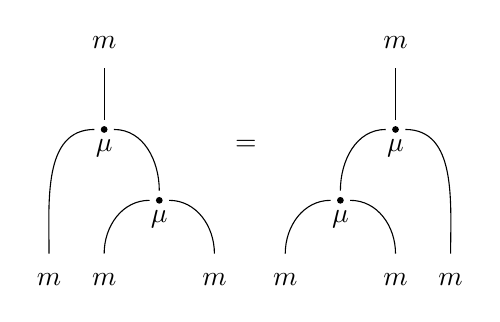
\begin{tikzpicture}
\def\delta{0.7}
\def\xa{0};
\def\xb{\delta};
\def\xc{\delta * 2};
\def\xd{\delta * 3};

\def \ya{0.8};
\def \yb{1.7};
\def \yc{2.6};

\node(a) at (\xa, 0) {};
\node(b) at (\xb, \yb) {};
\node(c) at (\xc, \ya) {};
\node(d) at (\xb, \yc) {};
\node(e) at (\xb, 0) {};
\node(f) at (\xd, 0) {};
\filldraw[black] (b) circle (1 pt);
\filldraw[black] (c) circle (1 pt);
\node [below] at (b) {$\mu$};
\draw (a) to [out=90, in=180]  node[left] {}(b);
\draw (c) to [out=90, in=0]  node[right] {} (b);
\draw (b) -- node[right] {} (d);
\draw (e) to [out=90, in=180]  node[left] {}(c);
\draw (f) to [out=90, in=0]  node[right] {}(c);
\node [below] at (c) {$\mu$};
\node [below] at (a) {$m$};
\node [above] at (d) {$m$};
\node [below] at (e) {$m$};
\node [below] at (f) {$m$};

\def\xe{2.5}
\node at (\xe, 1.5) {$=$};

\def\off{3}
\def\xa{\off + \delta * 0};
\def\xb{\off + \delta * 1};
\def\xc{\off + \delta * 2};
\def\xd{\off + \delta * 3};

\node(a) at (\xa, 0) {};
\node(b) at (\xc, 0) {};
\node(c) at (\xd, 0) {};
\node(d) at (\xb, \ya) {};
\node(e) at (\xc, \yb) {};
\node(f) at (\xc, \yc) {};
\filldraw[black] (d) circle (1 pt);
\filldraw[black] (e) circle (1 pt);
\node [below] at (d) {$\mu$};
\draw (a) to [out=90, in=180]  node[left] {}(d);
\draw (b) to [out=90, in=0]  node[right] {} (d);
\draw (e) -- node[right] {} (f);
\draw (d) to [out=90, in=180]  node[left] {}(e);
\draw (c) to [out=90, in=0]  node[right] {}(e);
\node [below] at (e) {$\mu$};
\node [below] at (a) {$m$};
\node [below] at (b) {$m$};
\node [below] at (c) {$m$};
\node [above] at (f) {$m$};
\end{tikzpicture}
\caption{Associativity law}
\label{fig-assoc}
\end{figure}

The important property of a string diagram is that, because of functoriality, its value---the compound morphism it represents---doesn't change under continuous transformations.

\subsection{Monoid}

First we'd like to show that the carrier of the free $h$-algebra $(m, \sigma)$ which, as we've seen before, is also the initial algebra for the list functor $I + h \otimes -$, is automatically a monoid. To show that, we need to define its unit and multiplication---two morphisms that satisfy monoid laws. The obvious candidate for unit is the universal mapping $\pi \colon I \to m$. It's the morphism in the definition of the free algebra from the previous post (see Fig \ref{fig-freei}). 

\begin{figure}[h]
\centering
\begin{tikzcd}
  & m
  \arrow[dd, bend left=30, "g"]
  \arrow[dl, "U"', leftarrow, dotted] \arrow[d, leftarrow, "\pi"'] \\
  (m, \sigma)
  \arrow[d, "g", dashed]
  & I 
  \arrow[d, "f"'] \\
  (n, \nu) 
  \arrow[r, "U", dotted]
  & n
\end{tikzcd}
\caption{Free $h$-algebra $(m, \sigma)$ generated by $I$}
\label{fig-freei}
\end{figure}


Multiplication is a morphism:
\[\mu \colon m \otimes m \to m\]
which, if you think of a free monoid as a list, is the generalization of list concatenation. 

The trick is to show that $m \otimes m$ is also a free $h$-algebra whose generator is $m$ itself. We could then use the universality of $m \otimes m$ to generate the unique algebra morphism from it to $m$ (which is also an $h$-algebra). That will be our $\mu$.

\begin{proposition}{Monoid.}

The free $h$-algebra $(m, \sigma)$ generated by the unit object $I$ is a monoid whose unit is:
\[\pi \colon I \to m\] 
and whose multiplication:
\[\mu \colon m \otimes m \to m\] 
is the unique $h$-algebra morphism 
\[(m \otimes m, \sigma \otimes m) \to (m, \sigma)\] 
induced by the identity morphism $id_m$.
\end{proposition}

\begin{proof}
In the previous post we've shown that, if $(m, \sigma)$ is a free algebra generated by the unit object $I$  with the universal map $\pi$, then $(m \otimes k, \sigma \otimes k)$ is a free algebra generated by $k$  with the universal map $\pi \otimes k$ (see Fig. \ref{fig-freek}).
\begin{figure}[H]
\centering
\begin{tikzcd}
  & m \otimes k
  \arrow[dd, bend left=40, "g"]
  \arrow[dl, "U"', leftarrow, dotted] \arrow[d, leftarrow, "\pi \otimes k"'] \\
  (m \otimes k, \sigma \otimes k)
  \arrow[d, "g", dashed]
  & k
  \arrow[d, "f"'] \\
  (n, \nu) 
  \arrow[r, "U", dotted]
  & n
\end{tikzcd}
\caption{Free $h$-algebra generated by $k \cong I \otimes k$}
\label{fig-freek}
\end{figure}

We get $\mu$ by redrawing this diagram: using $m$ as both the generator and the target algebra, and replacing $f$ with $id_m$ (see Fig. \ref{fig-monmul}):
\begin{figure}[H]
\centering
\begin{tikzcd}
  & m \otimes m
  \arrow[dd, bend left=40, "\mu"]
  \arrow[dl, "U"', leftarrow, dotted] \arrow[d, leftarrow, "\pi \otimes m"'] \\
  (m \otimes m, \sigma \otimes m)
  \arrow[d, "\mu", dashed]
  & m
  \arrow[d, "id_m"'] \\
  (m, \sigma) 
  \arrow[r, "U", dotted]
  & m
\end{tikzcd}
\caption{Monoid multiplication as an $h$-algebra morphism}
\label{fig-monmul}
\end{figure}

Since so defined $\mu$ is an $h$-algebra morphism, it makes the following diagram, Fig. \ref{fig-mualg}, commute.

\begin{figure}[H]
\centering
\begin{tikzcd}
  h \otimes m \otimes m
  \arrow[d, "h \otimes \mu"']
  \arrow[r, "\sigma \otimes m"]  
  & m \otimes m 
  \arrow[d, "\mu"] \\
  h \otimes m
  \arrow[r, "\sigma"]
  & m
\end{tikzcd}
\caption{$\mu$ is an $h$-algebra morphism}
\label{fig-mualg}
\end{figure}


This commuting condition can be redrawn as the identity of two string diagrams (Fig. \ref{fig-mualgmor}) corresponding to the two paths through the original diagram. 

\begin{figure}[H]
\centering
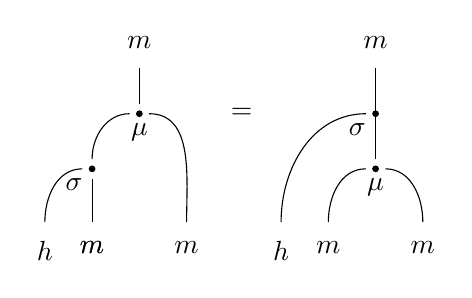
\begin{tikzpicture}
\def\dx{0.6}
\def\xa{0};
\def\xb{\dx};
\def\xc{\dx * 2};
\def\xd{\dx * 3};

\def \ya{0.8};
\def \yb{1.5};
\def \yc{2.2};

\node(h) at (\xa, 0) {};
\node(m1) at (\xb, 0) {};
\node(m2) at (\xd, 0) {};
\node(sig) at (\xb, \ya) {};
\node(mu) at (\xc, \yb) {};
\node(mt) at (\xc, \yc) {};
\filldraw[black] (sig) circle (1 pt);
\filldraw[black] (mu) circle (1 pt);
\node [below] at (m1) {$m$};
\node [below] at (mu) {$\mu$};
\node [below left] at (sig) {$\sigma$};
\draw (h) to [out=90, in=180] (sig);
\draw (m1) -- (sig);
\draw (m2)  to [out=90, in=0] (mu);
\draw (sig)  to [out=90, in=180] (mu);
\draw (mu) -- (mt);
\node[below] at (h) {$h$};
\node[below] at (m1) {$m$};
\node[below] at (m2) {$m$};
\node[above] at (mt) {$m$};

\def\off{3.0}
\def\xxa{\off + \xa};
\def\xxb{\off + \xb};
\def\xxc{\off + \xc};
\def\xxd{\off + \xd};

\node(hr) at (\xxa, 0) {};
\node(m1r) at (\xxb, 0) {};
\node(m2r) at (\xxd, 0) {};
\node(mur) at (\xxc, \ya) {};
\node(sigr) at (\xxc, \yb) {};
\node(mrt) at (\xxc, \yc) {};

\node at (\off - 0.5, 1.5) {$=$};

\filldraw[black] (mur) circle (1 pt);
\filldraw[black] (sigr) circle (1 pt);
\node [below] at (mur) {$\mu$};
\node [below left] at (sigr) {$\sigma$};
\draw (hr) to [out=90, in=180]  (sigr);
\draw (m1r) to [out=90, in=180]  (mur);
\draw (m2r) to [out=90, in=0]  (mur);
\node[below] at (hr) {$h$};
\node[below] at (m1r) {$m$};
\node[below] at (m2r) {$m$};
\node[above] at (mrt) {$m$};
\draw (mur) -- (sigr);
\draw (mur) -- (mrt);

\end{tikzpicture}
\caption{String diagram showing that $\mu$ is an algebra morphism}
\label{fig-mualgmor}
\end{figure}


The universal condition in Fig. \ref{fig-monmul}:
\[ \mu \circ (\pi \otimes m) = id_m \]
gives us immediately the left unit law for the monoid.

The right unit law:
\[\mu \circ (m \otimes \pi) = id_m \]
requires a little more work. 

There is a standard trick that we can use to show that two morphisms, whose source (in this case $m$) is a free algebra, are equal. It's enough to prove that they are algebra morphisms, and that they are both induced by the same morphism (in this case $\pi$). Their equality then follows from the uniqueness of the universal construction.

We know that $\mu$ is an algebra morphism so, if we can show that $m \otimes \pi$ is also an algebra morphism, their composition will be an algebra morphism too. Trivially, $id_m$ is an algebra morphism so, if we can show that the two are induced by the same regular morphism $\pi$, then they must be equal.

To show that $m \otimes \pi$ is an $h$-algebra morphism, we have to show that the diagram in Fig. \ref{fig-aalgmorpi} commutes.

\begin{figure}[H]
\centering
\begin{tikzcd}
  h \otimes m
  \arrow[r, "\sigma"]
  \arrow[d, "h \otimes m \otimes \pi"]
  & m
  \arrow[d, "m \otimes \pi"] \\
  h \otimes m \otimes m
  \arrow[r, "\sigma \otimes m"]
  & m \otimes m
\end{tikzcd}
\caption{$m \otimes \pi$ as an $h$-algebra morphism}
\label{fig-aalgmorpi}
\end{figure}

We can redraw the two paths through Fig. \ref{fig-aalgmorpi} as two string diagrams in Fig. \ref{fig-mpialgmor}. They are equal because they can be deformed into each other.

\begin{figure}[H]
\centering
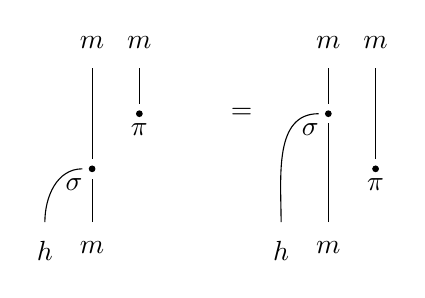
\begin{tikzpicture}
\def\dx{0.6}
\def\xa{0};
\def\xb{\dx};
\def\xc{\dx * 2};

\def \ya{0.8};
\def \yb{1.5};
\def \yc{2.2};

\node(a) at (\xa, 0) {};
\node(b) at (\xb, \ya) {};
\node(c) at (\xb, 0) {};
\node(d) at (\xb, \yc) {};
\node(e) at (\xc, \yb) {};
\node(f) at (\xc, \yc) {};
\filldraw[black] (e) circle (1 pt);
\node [below] at (e) {$\pi$};
\filldraw[black] (b) circle (1 pt);
\node [below left] at (b) {$\sigma$};
\draw (a) to [out=90, in=180] (b);
\draw (c) -- (b);
\draw (b) -- (d);
\draw (e) -- (f);
\node[below] at (a) {$h$};
\node[below] at (c) {$m$};
\node[above] at (d) {$m$};
\node[above] at (f) {$m$};

\def\off{3.0}
\def\xxa{\off + \xa};
\def\xxb{\off + \xb};
\def\xxc{\off + \xc};

\node(aa) at (\xxa, 0) {};
\node(bb) at (\xxb, \yb) {};
\node(cc) at (\xxb, 0) {};
\node(dd) at (\xxb, \yc) {};
\node(ee) at (\xxc, \ya) {};
\node(ff) at (\xxc, \yc) {};

\node at (\off - 0.5, 1.5) {$=$};

\filldraw[black] (ee) circle (1 pt);
\filldraw[black] (bb) circle (1 pt);
\node [below] at (ee) {$\pi$};
\node [below left] at (bb) {$\sigma$};
\draw (aa) to [out=90, in=180]  (bb);
\node[below] at (aa) {$h$};
\node[below] at (cc) {$m$};
\node[above] at (dd) {$m$};
\node[above] at (ff) {$m$};
\draw (cc) -- (bb);
\draw (bb) -- (dd);
\draw (ee) -- (ff);

\end{tikzpicture}
\caption{String diagram showing that $m \otimes \pi$ is an algebra morphism}
\label{fig-mpialgmor}
\end{figure}

Therefore the composition $\mu \circ (m \otimes \pi)$ is also an $h$-algebra morphism. The string diagram that illustrates this fact is shown in Fig. \ref{fig-mumpi}.

\begin{figure}[H]
\centering
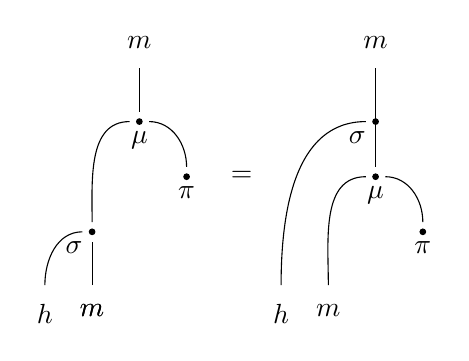
\begin{tikzpicture}
\def\dx{0.6}
\def\xa{0};
\def\xb{\dx};
\def\xc{\dx * 2};
\def\xd{\dx * 3};

\def \ya{0.8};
\def \yb{1.5};
\def \yc{2.2};
\def \yd{3.0};

\node(h) at (\xa, 0) {};
\node(m1) at (\xb, 0) {};
\node(pi) at (\xd, \yb) {};
\node(sig) at (\xb, \ya) {};
\node(mu) at (\xc, \yc) {};
\node(mt) at (\xc, \yd) {};
\filldraw[black] (sig) circle (1 pt);
\filldraw[black] (mu) circle (1 pt);
\filldraw[black] (pi) circle (1 pt);
\node [below] at (m1) {$m$};
\node [below] at (mu) {$\mu$};
\node [below] at (pi) {$\pi$};
\node [below left] at (sig) {$\sigma$};
\draw (h) to [out=90, in=180] (sig);
\draw (m1) -- (sig);
\draw (pi)  to [out=90, in=0] (mu);
\draw (sig)  to [out=90, in=180] (mu);
\draw (mu) -- (mt);
\node[below] at (h) {$h$};
\node[below] at (m1) {$m$};
\node[above] at (mt) {$m$};

\def\off{3.0}
\def\xxa{\off + \xa};
\def\xxb{\off + \xb};
\def\xxc{\off + \xc};
\def\xxd{\off + \xd};

\node(hr) at (\xxa, 0) {};
\node(m1r) at (\xxb, 0) {};
\node(pir) at (\xxd, \ya) {};
\node(mur) at (\xxc, \yb) {};
\node(sigr) at (\xxc, \yc) {};
\node(mrt) at (\xxc, \yd) {};

\node at (\off - 0.5, 1.5) {$=$};

\filldraw[black] (mur) circle (1 pt);
\filldraw[black] (sigr) circle (1 pt);
\filldraw[black] (pir) circle (1 pt);
\node [below] at (mur) {$\mu$};
\node [below left] at (sigr) {$\sigma$};
\draw (hr) to [out=90, in=180]  (sigr);
\draw (m1r) to [out=90, in=180]  (mur);
\draw (pir) to [out=90, in=0]  (mur);
\node[below] at (hr) {$h$};
\node[below] at (m1r) {$m$};
\node[below] at (pir) {$\pi$};
\node[above] at (mrt) {$m$};
\draw (mur) -- (sigr);
\draw (mur) -- (mrt);

\end{tikzpicture}
\caption{String diagram showing that $\mu \circ (m \otimes \pi)$ is an algebra morphism}
\label{fig-mumpi}
\end{figure}


Since the identity $h$-algebra morphism is induced by $\pi$, we'd like to show that $\mu \circ (m \otimes \pi)$  is also induced by $\pi$ (Fig. \ref{fig-unitlaw}). 

\begin{figure}[H]
\centering
\begin{tikzcd}
  & m
  \arrow[dd, bend left=30, "\mu \circ (m \otimes \pi)"]
  \arrow[dl, "U"', leftarrow, dotted] \arrow[d, leftarrow, "\pi"'] \\
  (m, \sigma)
  \arrow[d, "\mu \circ (m \otimes \pi)"', dashed]
  & I 
  \arrow[d, "\pi"'] \\
  (m, \sigma)
  \arrow[r, "U", dotted]
  & m
\end{tikzcd}
\caption{Universal property of the free $h$-algebra generated by $I$, with the algebra morphism induced by $\pi$}
\label{fig-unitlaw}
\end{figure}

To do that, we have to prove the universal condition in Fig. \ref{fig-unitlaw}:
\[\mu \circ (m \otimes \pi) \circ \pi = \pi\]

This is represented as a string diagram identity in Fig. \ref{fig-refl}. We can deform this diagram by sliding the left $\pi$ node up, past the right $\pi$ node, and then using the left identity.
\begin{figure}[H]
\centering
\begin{tikzpicture}
\def\dx{0.5}
\def\xa{0};
\def\xb{\dx};
\def\xc{\dx * 2};
\def\xd{\dx * 3};

\def \ya{0.8};
\def \yb{1.5};
\def \yc{2.2};
\def \yd{3};

\node(pi1) at (\xa, \ya) {};
\node(pi2) at (\xc, \yb) {};
\node(mu) at (\xb, \yc) {};
\node(m) at (\xb, \yd) {};
\filldraw[black] (pi1) circle (1 pt);
\filldraw[black] (mu) circle (1 pt);
\node [below] at (pi1) {$\pi$};
\filldraw[black] (pi2) circle (1 pt);
\node [below] at (pi2) {$\pi$};
\draw (pi1)  to [out=90, in=180]  (mu);
\draw (pi2)  to [out=90, in=0]   (mu);
\draw (mu) -- (m);
\node[below] at (mu) {$\mu$};
\node[above] at (m) {$m$};

\def\off{3}
\node at (\off - 1, 1.5) {$=$};

\def\xa{\off};

\node(pi) at (\xa, \ya) {};
\node(m) at (\xa, \yd) {};


\filldraw[black] (pi) circle (1 pt);
\node [below] at (pi) {$\pi$};
\node[above] at (m) {$m$};
\draw (pi) -- (m);

\end{tikzpicture}
\caption{Universal condition in Fig. \ref{fig-unitlaw}.}
\label{fig-refl}
\end{figure}

This concludes the proof of the right identity.

The proof of associativity is very similar, so I'll just sketch it. We have to show that the two diagrams in Fig. \ref{fig-assoc} are equal. We'll use the same trick as before. We'll show that they are both algebra morphisms. Their source is a free algebra generated by $m \otimes m$ (see Fig. \ref{fig-monassoc}---the other diagram has $\mu \circ (\mu \otimes m)$ replaced by $\mu \circ (m \otimes \mu)$). The universal condition follows from the unit law for $m$. Associativity condition:
\[\mu \circ (\mu \otimes m) = \mu \circ (m \otimes \mu)\]
will then follow from the uniqueness of the universal construction.
\begin{figure}[H]
\centering
\begin{tikzcd}
  & m \otimes m \otimes m
  \arrow[dd, bend left=40, "\mu \circ (\mu \otimes m)"]
  \arrow[dl, "U"', leftarrow, dotted] 
  \arrow[d, leftarrow, "\pi \otimes m \otimes m"'] \\
  (m \otimes m \otimes m, \sigma \otimes m \otimes m)
  \arrow[d, "\mu \circ (\mu \otimes m)", dashed]
  & m \otimes m
  \arrow[d, "\mu"'] \\
  (m, \sigma) 
  \arrow[r, "U", dotted]
  & m
\end{tikzcd}
\caption{One part of associativity as an $h$-algebra morphism}
\label{fig-monassoc}
\end{figure}

You can easily convince yourself that showing that something is an $h$-algebra morphism can be done by first attaching the $h$ leg to the left of the string diagram and then sliding it to the top of the diagram, as illustrated in Fig. \ref{fig-algassoc}. This can be accomplished by repeatedly using the fact that $\mu$ is an $h$-algebra morphism.

\begin{figure}[H]
\centering
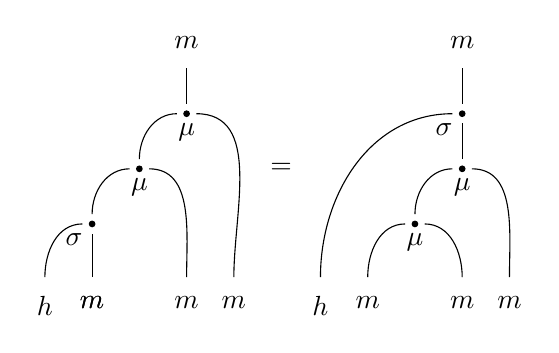
\begin{tikzpicture}
\def\dx{0.6}
\def\xa{0};
\def\xb{\dx};
\def\xc{\dx * 2};
\def\xd{\dx * 3};
\def\xe{\dx * 4};

\def \ya{0.8};
\def \yb{1.5};
\def \yc{2.2};
\def \yd{2.9};

\node(h) at (\xa, 0) {};
\node(m1) at (\xb, 0) {};
\node(m2) at (\xd, 0) {};
\node(m3) at (\xe, 0) {};
\node(sig) at (\xb, \ya) {};
\node(mu) at (\xc, \yb) {};
\node(mu2) at (\xd, \yc) {};
\node(mt) at (\xd, \yd) {};
\filldraw[black] (sig) circle (1 pt);
\filldraw[black] (mu) circle (1 pt);
\filldraw[black] (mu2) circle (1 pt);
\node [below] at (m1) {$m$};
\node [below] at (mu) {$\mu$};
\node [below] at (mu2) {$\mu$};
\node [below left] at (sig) {$\sigma$};
\draw (h) to [out=90, in=180] (sig);
\draw (m1) -- (sig);
\draw (m2)  to [out=90, in=0] (mu);
\draw (m3)  to [out=90, in=0] (mu2);
\draw (sig)  to [out=90, in=180] (mu);
\draw (mu)  to [out=90, in=180] (mu2);
\draw (mu2) -- (mt);
\node[below] at (h) {$h$};
\node[below] at (m1) {$m$};
\node[below] at (m2) {$m$};
\node[below] at (m3) {$m$};
\node[above] at (mt) {$m$};

\def\off{3.5}
\def\xxa{\off + \xa};
\def\xxb{\off + \xb};
\def\xxc{\off + \xc};
\def\xxd{\off + \xd};
\def\xxe{\off + \xe};

\node(hr) at (\xxa, 0) {};
\node(m1r) at (\xxb, 0) {};
\node(m2r) at (\xxd, 0) {};
\node(m3r) at (\xxe, 0) {};
\node(mur) at (\xxc, \ya) {};
\node(mur2) at (\xxd, \yb) {};
\node(sigr) at (\xxd, \yc) {};
\node(mrt) at (\xxd, \yd) {};

\node at (\off - 0.5, 1.5) {$=$};

\filldraw[black] (mur) circle (1 pt);
\filldraw[black] (mur2) circle (1 pt);
\filldraw[black] (sigr) circle (1 pt);
\node [below] at (mur) {$\mu$};
\node [below] at (mur2) {$\mu$};
\node [below left] at (sigr) {$\sigma$};
\draw (hr) to [out=90, in=180]  (sigr);
\draw (mur) to [out=90, in=180]  (mur2);
\draw (m1r) to [out=90, in=180]  (mur);
\draw (m2r) to [out=90, in=0]  (mur);
\draw (m3r) to [out=90, in=0]  (mur2);
\node[below] at (hr) {$h$};
\node[below] at (m1r) {$m$};
\node[below] at (m2r) {$m$};
\node[below] at (m3r) {$m$};
\node[above] at (mrt) {$m$};
\draw (mur2) -- (sigr);
\draw (sigr) -- (mrt);

\end{tikzpicture}
\caption{String diagram showing that one of the associativity diagrams is an $h$-algebra morphism}
\label{fig-algassoc}
\end{figure}

The same process can be applied to the second associativity diagram, thus completing the proof.

\end{proof}

For Haskell programmers, recall from the previous post our construction of the free $h$-algebra generated by $k$ and the derivation of the algebra morphism $g$ from it to the internal-hom algebra:

\begin{haskell}
g :: Expr -> (k -> n)
g () = f
g a  = \k -> nu (a, f k)
g (a, b) = \k -> nu (a, nu (b, f k))
.dot.dot.dot
\end{haskell}
In the current proof we have replaced $k$ with $m$, which generalizes the list of $h$s, $f$ became $id$, and $\nu$ is a function that prepends an element to a list. In other words, $g$ concatenates its list-argument in front of the second list, and it does it in the correct order.

\subsection{Free Monoid}

The monoid whe have just constructed from the free algebra is a free monoid. As we did with free algebras, instead of using the free/forgetful adjunction to prove it, we'll use the free-object universal construction. 

\begin{theorem}{Free Monoid.}

The monoid $(m, \pi, \mu)$ is a \textit{free} monoid generated by $h$, with a universal mapping given by $u = \sigma \circ (h \otimes \pi)$:
\[\begin{tikzcd}
  u \colon h
  \arrow[r, "h \otimes \pi"]
  & h \otimes m
  \arrow[r, "\sigma"]
  & m
\end{tikzcd}\]

That is, for any monoid $(n, \eta, \nu)$ and any morphism $s \colon h \to n$, there is a unique \textit{monoid morphism} $t$ from $(m, \pi, \mu)$ to $(n, \eta, \nu)$ such that the universal condition holds:
\[t \circ u = s\]
(see Fig. \ref{fig-freemon}).
\begin{figure}[H]
\centering
\begin{tikzcd}
  & m
  \arrow[dd, bend left=40, "t"]
  \arrow[dl, "U"', leftarrow, dotted] 
  \arrow[d, leftarrow, "u"'] \\
  (m, \pi, \mu)
  \arrow[d, "t", dashed]
  & h
  \arrow[d, "s"'] \\
  (n, \eta, \nu) 
  \arrow[r, "U", dotted]
  & n
\end{tikzcd}
\caption{Free monoid diagram}
\label{fig-freemon}
\end{figure}
\end{theorem}

\begin{proof} Recall that $(m, \sigma)$ is a free $h$-algebra generated by $I$. It turns out that any monoid $(n, \eta, \nu)$, for which there is a morphism $s \colon h \to n$, is automatically a carrier of an $h$-algebra. We construct its structure map $\lambda$ by combining $s$ with monoid multiplication $\nu$:
\[\begin{tikzcd}
  \lambda \colon h \otimes n
  \arrow[r, "s \otimes n"]
  & n \otimes n
  \arrow[r, "\nu"]
  & n
\end{tikzcd}\]

We can use $n$'s monoidal unit $\eta$ to insert $I$ into $n$. Because $(m, \sigma)$ is a free $h$-algebra, there is a unique algebra morphism, let's call it $t$, from it to $(n, \lambda)$, which is induced by $\eta$, such that $t \circ \pi = \eta$ (see Fig. \ref{fig-freemonalg}). We want to show that this algebra morphism is also a \textit{monoid morphism}. Furthermore, if we can show that this is the \textit{unique} monoid morphism induced by $s$, we will have a proof that $m$ is a free monoid.

\begin{figure}[H]
\centering
\begin{tikzcd}
  & m
  \arrow[dd, bend left=40, "t"]
  \arrow[dl, "U"', leftarrow, dotted] 
  \arrow[d, leftarrow, "\pi"'] \\
  (m, \sigma)
  \arrow[d, "t", dashed]
  & I
  \arrow[d, "\eta"'] \\
  (n, \lambda) 
  \arrow[r, "U", dotted]
  & n
\end{tikzcd}
\caption{Algebra morphism between monoids}
\label{fig-freemonalg}
\end{figure}

Since $t$ is an algebra morphism, the rectangle in Fig. \ref{fig-aalgmort} commutes. 

\begin{figure}[H]
\centering
\begin{tikzcd}
  h \otimes m
  \arrow[rr, "\sigma"]
  \arrow[d, "h \otimes t"']
  & & m
  \arrow[d, "t"] \\
  h \otimes n
  \arrow[rr, bend right=40, "\lambda"]
  \arrow[r, "s \otimes n"']
  & n \otimes n
  \arrow[r, "\nu"']
  & n
\end{tikzcd}
\caption{$t$ is an $h$-algebra morphism}
\label{fig-aalgmort}
\end{figure}


Let's redraw it as an identity of string diagrams, Fig. \ref{fig-algmon}. We'll make use of it in a moment.

\begin{figure}[H]
\centering
\begin{tikzpicture}
\def\dx{0.6}
\def\dy{0.8}

\def\xa{0};
\def\xb{\dx};
\def\xc{2 * \dx};

\def \ya{0};
\def \yb{\dy};
\def \yc{2 * \dy};
\def \yd{3 * \dy};

\node(h) at (\xa, \ya) {};
\node(m) at (\xc, \ya) {};
\node(s) at (\xa, \yb + 0.2) {};
\node(t) at (\xc, \yb - 0.2) {};
\node(nu) at (\xb, \yc) {};
\node(n) at (\xb, \yd) {};

\filldraw[black] (s) circle (1 pt);
\filldraw[black] (t) circle (1 pt);
\filldraw[black] (nu) circle (1 pt);

\node [left] at (s) {$s$};
\node [right] at (t) {$t$};
\node [below] at (nu) {$\nu$};

\draw (h) -- (s);
\draw (m) -- (t);
\draw (s) to [out=90, in=180]  node[left] {$n$} (nu);
\draw (t) to [out=90, in=0]   node[right] {$n$} (nu);
\draw (nu) -- (n);
\node[below] at (a) {$h$};
\node[below] at (m) {$m$};
\node[above] at (n) {$n$};

\def\yy{\yb + 0.5 * \dy}
\node at (2.2, \yy) {$=$};

\def\xx{3}

\def\xxa{\xx};
\def\xxb{\xx + \xb};
\def\xxc{\xx + \xc};

\node(aa) at (\xxa, \ya) {};
\node(bb) at (\xxc, \ya) {};
\node(cc) at (\xxa, \yb) {};
\node(dd) at (\xxc, \yb) {};
\node(ee) at (\xxc, \yb) {};
\node(ff) at (\xxc, \yd) {};
\node(gg) at (\xxc, \yc) {};

\filldraw[black] (ee) circle (1 pt);
\filldraw[black] (gg) circle (1 pt);

\node [right] at (gg) {$t$};
\node [below left] at (ee) {$\sigma$};

\draw (aa) to [out=90, in=180] (ee);
\draw (bb) -- (ee);
\draw (ee) -- node[right] {$m$} (gg);
\draw (gg) -- (ff);
\node[below] at (aa) {$h$};
\node[below] at (bb) {$m$};
\node[above] at (ff) {$n$};

\end{tikzpicture}
\caption{$t$ is an $h$-algebra morphism}
\label{fig-algmon}
\end{figure}

Going back to Fig. \ref{fig-freemon}, we want to show that the universal condition holds, which means that we want the diagram in Fig. \ref{fig-unift} to commute (I have expanded the definition of $u$).

\begin{figure}[H]
\centering
\begin{tikzcd}
  h
  \arrow[rr, bend left=40, "u"]
  \arrow[r, "h \otimes \pi"]
  \arrow[rd, "s"']
  & h \otimes m 
  \arrow[r, "\sigma"]
  & m
  \arrow[ld, "t"] \\
  & n
\end{tikzcd}
\caption{Free monoid universal condition}
\label{fig-unift}
\end{figure}

In other words we want show that the following two string diagrams are equal:

\begin{figure}[H]
\centering
\begin{tikzpicture}
\def\dx{0.6}
\def\xa{0};
\def\xb{\dx};
\def\xc{\dx * 2};

\def\dy{0.8}
\def \ya{0};
\def \yb{\dy};
\def \yc{2 * \dy};
\def \yd{3 * \dy};
\def \ye{4 * \dy};

\node(a) at (\xb, \ya) {};
\node(b) at (\xc, \yb) {};
\node(c) at (\xc, \yc) {};
\node(d) at (\xc, \yd) {};
\node(e) at (\xc, \ye) {};
\filldraw[black] (b) circle (1 pt);
\filldraw[black] (c) circle (1 pt);
\filldraw[black] (d) circle (1 pt);
\node [below] at (a) {$h$};
\node [below] at (b) {$\pi$};
\node [below left] at (c) {$\sigma$};
\node [left] at (d) {$t$};
\node [above] at (e) {$n$};
\draw (a) to [out=90, in=180] (c);
\draw (b) --  node[right] {$m$} (c);
\draw (c) -- node[right] {$m$} (d);
\draw (d) -- (e);

\def\xd{2.2}
\def\xe{3.2}
\node at (\xd, 1.5) {$=$};
\node(e) at (\xe, 0) {};
\node(f) at (\xe, \yc) {};
\node(g) at (\xe, \ye) {};
\filldraw[black] (f) circle (1 pt);
\node [left] at (f) {$s$};
\draw (e) -- (f);
\draw (f) -- (g);
\node [below] at (e) {$h$};
\node [above] at (g) {$n$};
\end{tikzpicture}
\caption{Free monoid universal condition}
\label{fig-struni}
\end{figure}

Using the identity in Fig. \ref{fig-algmon}, the left hand side can be rewritten as:

\begin{figure}[H]
\centering
\begin{tikzpicture}
\def\dx{0.6}
\def\xa{0};
\def\xb{\dx};
\def\xc{\dx * 2};

\def\dy{0.8}
\def \ya{0};
\def \yb{\dy};
\def \yc{2 * \dy};
\def \yd{3 * \dy};
\def \ye{4 * \dy};
\def \yf{5 * \dy};

\node(a) at (\xa, \ya) {};
\node(b) at (\xc, \yb) {};
\node(c) at (\xa, \yc) {};
\node(d) at (\xc, \yc) {};
\node(e) at (\xb, \yd) {};
\node(f) at (\xb, \ye) {};
\node(g) at (\xb, \yf) {};
\filldraw[black] (b) circle (1 pt);
\filldraw[black] (c) circle (1 pt);
\filldraw[black] (d) circle (1 pt);
\filldraw[black] (e) circle (1 pt);
\node [below] at (a) {$h$};
\node [below] at (b) {$\pi$};
\node [below] at (e) {$\nu$};
\node [left] at (c) {$s$};
\node [left] at (d) {$t$};
\node [above] at (f) {$n$};
\draw (a) -- (c);
\draw (b) -- (d);

\draw (c) to [out=90, in=180] node[left] {$n$} (e);
\draw (d) to [out=90, in=0] node[right] {$n$} (e);
\draw (e) -- (f);

\end{tikzpicture}
\caption{Step 1 in transforming Fig \ref{fig-struni}}
\label{fig-}
\end{figure}

The right leg can be shrunk down to $\eta$ using the universal condition in Fig. \ref{fig-freemonalg}:
\[t \circ \pi = \eta\]
which, incidentally, also expresses the fact that $t$ preserves the monoidal unit.

Finally, we can use the right unit law for the monoid $n$, Fig. \ref{fig-runitn},

\begin{figure}[H]
\centering
\begin{tikzpicture}
\def\dx{0.6}
\def\xa{0};
\def\xb{\dx};
\def\xc{\dx * 2};

\def \ya{0.8};
\def \yb{1.7};
\def \yc{2.6};

\node(a) at (\xa, 0) {};
\node(b) at (\xb, \yb) {};
\node(c) at (\xc, \ya) {};
\node(d) at (\xb, \yc) {};
\filldraw[black] (b) circle (1 pt);
\node [below] at (c) {$\eta$};
\node [below] at (a) {$n$};
\node [above] at (d) {$n$};
\filldraw[black] (c) circle (1 pt);
\node [below] at (b) {$\nu$};
\draw (a) to [out=90, in=180]  (b);
\draw (c) to [out=90, in=0]  node[right] {$n$} (b);
\draw (b) -- (d);

\def\xd{3.5}
\def\xe{2.5}
\node(e) at (\xd, 0) {};
\node(f) at (\xd, \yc) {};
\node at (\xe, 1.5) {$=$};
\draw (e) -- (f);
\node [below] at (e) {$n$};
\node [above] at (f) {$n$};
\end{tikzpicture}
\caption{Right unit law for monoid $n$}
\label{fig-runitn}
\end{figure}
to arrive at the right hand side of the identity in Fig. \ref{fig-struni}. This completes the proof of the universal condition in Fig. \ref{fig-freemon}. 

Now we have to show that $t$ is a full-blown monoid morphism, that is, it preserves multiplication (Fig. \ref{fig-mul}).

\begin{figure}[H]
\centering
\begin{tikzcd}
  m \otimes m
  \arrow[r, "t \otimes t"]
  \arrow[d, "\mu"]
  & n \otimes n
  \arrow[d, "\nu"] \\
  m
  \arrow[r, "t"]
  & n
\end{tikzcd}
\caption{Preservation of multiplication}
\label{fig-mul}
\end{figure}

The corresponding string diagrams are shown in Fig. \ref{fig-presmul}.

\begin{figure}[H]
\centering
\begin{tikzpicture}
\def\dx{0.6}
\def\dy{0.8}

\def\xa{0};
\def\xb{\dx};
\def\xc{2 * \dx};

\def \ya{0};
\def \yb{\dy};
\def \yc{2 * \dy};
\def \yd{3 * \dy};

\node(m1) at (\xa, \ya) {};
\node(m2) at (\xc, \ya) {};
\node(t1) at (\xa, \yb) {};
\node(t2) at (\xc, \yb) {};
\node(nu) at (\xb, \yc) {};
\node(n) at (\xb, \yd) {};

\filldraw[black] (t1) circle (1 pt);
\filldraw[black] (t2) circle (1 pt);
\filldraw[black] (nu) circle (1 pt);

\node [left] at (t1) {$t$};
\node [right] at (t2) {$t$};
\node [below] at (nu) {$\nu$};

\draw (m1) -- (t1);
\draw (m2) -- (t2);
\draw (t1) to [out=90, in=180]  node[left] {$n$} (nu);
\draw (t2) to [out=90, in=0]   node[right] {$n$} (nu);
\draw (nu) -- (n);
\node[below] at (m1) {$m$};
\node[below] at (m2) {$m$};
\node[above] at (n) {$n$};

\node at (2.5, \yc) {$=$};

\def\xa{3.6};
\def\xb{\xa + \dx};
\def\xc{\xa + 2 * \dx};

\node(m1) at (\xa, \ya) {};
\node(m2) at (\xc, \ya) {};
\node(t) at (\xb, \yc) {};
\node(mu) at (\xb, \yb) {};
\node(n) at (\xb, \yd) {};

\filldraw[black] (t) circle (1 pt);
\filldraw[black] (mu) circle (1 pt);

\node [right] at (t) {$t$};
\node [below] at (mu) {$\mu$};

\node[below] at (m1) {$m$};
\node[below] at (m2) {$m$};
\node[above] at (n) {$n$};

\draw (m1) to [out=90, in=180] (mu);
\draw (m2) to [out=90, in=0]   (mu);
\draw (mu) -- node[left] {$m$} (t);
\draw (t) -- (n);

\end{tikzpicture}
\caption{Preservation of multiplication}
\label{fig-presmul}
\end{figure}



Let's start with the fact that $m \otimes m$ is the free $h$-algebra generated by $m$. We will show that the two paths through the diagram in Fig. \ref{fig-mul} are both $h$-algebra morphisms, and that they are induced by the same regular morphism $t \colon m \to n$. Therefore they must be equal. 

The bottom path in Fig. \ref{fig-mul}, $t \circ \mu$, is an $h$-algebra morphism by virtue of being a composition of two $h$-algebra morphisms. This composite is induced by morphism $t$ in the diagram Fig. \ref{fig-monmul1}.
\begin{figure}[H]
\centering
\begin{tikzcd}
  & m \otimes m
  \arrow[dd, bend left=40, "t \circ \mu"]
  \arrow[dl, "U"', leftarrow, dotted] \arrow[d, leftarrow, "\pi \otimes m"'] \\
  (m \otimes m, \sigma \otimes m)
  \arrow[d, "t \circ \mu", dashed]
  & m
  \arrow[d, "t"'] \\
  (n, \lambda) 
  \arrow[r, "U", dotted]
  & n
\end{tikzcd}
\caption{$h$-algebra morphism $t \circ \mu$}
\label{fig-monmul1}
\end{figure}

The universal condition in Fig. \ref{fig-monmul1} follows from the diagram in Fig. \ref{fig-uni1}, which follows from the left unit law for the monoid $(m, \pi, \mu)$.

\begin{figure}[H]
\centering
\begin{tikzpicture}
\def\dx{0.6}
\def\xa{0};
\def\xb{\dx};
\def\xc{\dx * 2};

\def\dy{0.8}
\def \ya{0};
\def \yb{\dy};
\def \yc{2 * \dy};
\def \yd{3 * \dy};
\def \ye{4 * \dy};

\node(m) at (\xc, \ya) {};
\node(pi) at (\xa, \yb) {};
\node(mu) at (\xb, \yc) {};
\node(t) at (\xb, \yd) {};
\node(n) at (\xb, \ye) {};

\filldraw[black] (pi) circle (1 pt);
\filldraw[black] (mu) circle (1 pt);
\filldraw[black] (t) circle (1 pt);

\node [below] at (m) {$m$};
\node [below] at (pi) {$\pi$};
\node [below left] at (mu) {$\mu$};
\node [left] at (t) {$t$};
\node [above] at (n) {$n$};

\draw (m)  to [out=90, in=0] (mu);
\draw (pi)  to [out=90, in=180] (mu);
\draw (mu) -- node[right] {$m$} (t);
\draw (t) -- (n);

\def\xd{2.2}
\def\xe{3.2}
\node at (\xd, 1.5) {$=$};
\node(m2) at (\xe, 0) {};
\node(t2) at (\xe, \yd) {};
\node(n2) at (\xe, \ye) {};
\filldraw[black] (t2) circle (1 pt);
\node [left] at (t2) {$t$};
\draw (m2) -- (t2);
\draw (t2) -- (n2);
\node [below] at (m2) {$m$};
\node [above] at (n2) {$n$};
\end{tikzpicture}
\caption{Universal condition in Fig. \ref{fig-monmul1}}
\label{fig-uni1}
\end{figure}

We want to show that the top path in Fig. \ref{fig-mul} is also an $h$-algebra morphism, that is, the diagram in Fig. \ref{fig-multop} commutes.

\begin{figure}[H]
\centering
\begin{tikzcd}
  h \otimes m \otimes m
  \arrow[r, "h \otimes t \otimes t"]
  \arrow[dd, "\sigma \otimes m"]
  & h \otimes n \otimes n
  \arrow[r, "h \otimes \nu"]
  & h \otimes n 
  \arrow[d, "s \otimes n"'] 
  \arrow[dd, bend left=40, "\lambda"]\\
  &
  & n \otimes n
  \arrow[d, "\nu"']
  \\
  m \otimes m
  \arrow[r, "t \otimes t"]
  & n \otimes n
  \arrow[r, "\nu"]
  & n
\end{tikzcd}
\caption{$h$-algebra morphism diagram for $\nu \circ (t \otimes t)$}
\label{fig-multop}
\end{figure}

We can redraw this diagram as a string diagram identity in Fig. \ref{fig-almornutt}.

\begin{figure}[H]
\centering
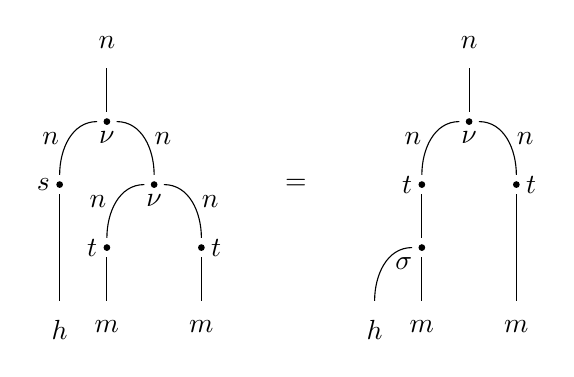
\begin{tikzpicture}
\def\dx{0.6}
\def\dy{0.8}

\def\xa{0};
\def\xb{\dx};
\def\xc{2 * \dx};
\def\xd{3 * \dx};

\def \ya{0};
\def \yb{\dy};
\def \yc{2 * \dy};
\def \yd{3 * \dy};
\def \ye{4 * \dy};

\node(h) at (\xa, \ya) {};
\node(m1) at (\xb, \ya) {};
\node(m2) at (\xd, \ya) {};
\node(t1) at (\xb, \yb) {};
\node(t2) at (\xd, \yb) {};
\node(nu1) at (\xc, \yc) {};
\node(f) at (\xa, \yc) {};
\node(nu2) at (\xb, \yd) {};
\node(n) at (\xb, \ye) {};

\filldraw[black] (t1) circle (1 pt);
\filldraw[black] (t2) circle (1 pt);
\filldraw[black] (nu1) circle (1 pt);
\filldraw[black] (nu2) circle (1 pt);
\filldraw[black] (f) circle (1 pt);

\node [left] at (t1) {$t$};
\node [right] at (t2) {$t$};
\node [left] at (f) {$s$};
\node [below] at (nu1) {$\nu$};
\node [below] at (nu2) {$\nu$};
\node [above] at (n) {$n$};
\node [below] at (h) {$h$};
\node [below] at (m1) {$m$};
\node [below] at (m2) {$m$};

\draw (t1) to [out=90, in=180]  node[left] {$n$} (nu1);
\draw (t2) to [out=90, in=0]   node[right] {$n$} (nu1);
\draw (f) to [out=90, in=180]  node[left] {$n$} (nu2);
\draw (nu1) to [out=90, in=0]   node[right] {$n$} (nu2);

\draw (h) -- (f);
\draw (m1) -- (t1);
\draw (m2) -- (t2);
\draw (nu2) -- (n);

\node at (3, \yc) {$=$};

\def\xa{4};
\def\xb{\xa + \dx};
\def\xc{\xa + 2 * \dx};
\def\xd{\xa + 3 * \dx};

\node(h) at (\xa, \ya) {};
\node(m1) at (\xb, \ya) {};
\node(m2) at (\xd, \ya) {};
\node(t1) at (\xb, \yc) {};
\filldraw[black] (t1) circle (1 pt);
\node [left] at (t1) {$t$};
\node(t2) at (\xd, \yc) {};
\filldraw[black] (t2) circle (1 pt);
\node [right] at (t2) {$t$};
\node(nu) at (\xc, \yd) {};
\filldraw[black] (nu) circle (1 pt);
\node [below] at (nu) {$\nu$};
\node(n) at (\xc, \ye) {};

\node [below] at (h) {$h$};
\node [below] at (m1) {$m$};
\node [below] at (m2) {$m$};
\node [above] at (n) {$n$};

\node(sigma) at (\xb, \yb) {};
\filldraw[black] (sigma) circle (1 pt);
\node [below left] at (sigma) {$\sigma$};

\draw (h) to [out=90, in=180](sigma);
\draw (m1) -- (sigma);
\draw (sigma) -- (t1);
\draw (m2) -- (t2);
\draw (nu) -- (n);

\draw (t1) to [out=90, in=180]  node[left] {$n$} (nu);
\draw (t2) to [out=90, in=0]   node[right] {$n$} (nu);

\end{tikzpicture}
\caption{$h$-algebra morphism diagram for $\nu \circ (t \otimes t)$}
\label{fig-almornutt}
\end{figure}

First, let's use the associativity law for the monoid $n$ to transform the left hand side. We get the diagram in Fig. \ref{fig-almornutt2}.


\begin{figure}[H]
\centering
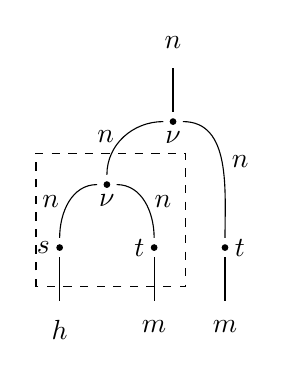
\begin{tikzpicture}
\def\dx{0.6}
\def\dy{0.8}

\def\xa{0};
\def\xb{\dx};
\def\xc{2 * \dx};
\def\xd{2.4 * \dx};
\def\xe{3.5 * \dx};

\def \ya{0};
\def \yb{\dy};
\def \yc{2 * \dy};
\def \yd{3 * \dy};
\def \ye{4 * \dy};

\node(h) at (\xa, \ya) {};
\node(m1) at (\xc, \ya) {};
\node(m2) at (\xe, \ya) {};
\node(t1) at (\xc, \yb) {};
\node(t2) at (\xe, \yb) {};
\node(nu2) at (\xd, \yd) {};
\node(f) at (\xa, \yb) {};
\node(nu1) at (\xb, \yc) {};
\node(n) at (\xd, \ye) {};

\filldraw[black] (t1) circle (1 pt);
\filldraw[black] (t2) circle (1 pt);
\filldraw[black] (nu1) circle (1 pt);
\filldraw[black] (nu2) circle (1 pt);
\filldraw[black] (f) circle (1 pt);

\node [left] at (t1) {$t$};
\node [right] at (t2) {$t$};
\node [left] at (f) {$s$};
\node [below] at (nu1) {$\nu$};
\node [below] at (nu2) {$\nu$};
\node [above] at (n) {$n$};
\node [below] at (h) {$h$};
\node [below] at (m1) {$m$};
\node [below] at (m2) {$m$};

\draw (f) to [out=90, in=180]  node[left] {$n$} (nu1);
\draw (t1) to [out=90, in=0]   node[right] {$n$} (nu1);
\draw (nu1) to [out=90, in=180]  node[left] {$n$} (nu2);
\draw (t2) to [out=90, in=0]   node[right] {$n$} (nu2);

\draw (h) -- (f);
\draw (m1) -- (t1);
\draw (m2) -- (t2);
\draw (nu2) -- (n);

\draw[dashed] (\xa - 0.3, \ya + 0.3) rectangle (\xc + 0.4, \yc + 0.4);


\end{tikzpicture}
\caption{After applying associativity, we can apply Fig. \ref{fig-algmon}}
\label{fig-almornutt2}
\end{figure}

We can now apply the identity in Fig. \ref{fig-algmon} to reproduce the right hand side of Fig. \ref{fig-almornutt}.

We have thus shown that both paths in Fig. \ref{fig-mul} are algebra morphisms. We know that the bottom path is induced by morphism $t$. What remains is to show that the top path, which is given by $\nu \circ (t \otimes t)$ is induced by the same $t$. This will be true, if we can show the universal condition in Fig. \ref{fig-monmul2}.


\begin{figure}[H]
\centering
\begin{tikzcd}
  & m \otimes m
  \arrow[dd, bend left=40, "\nu \circ (t \otimes t)"]
  \arrow[dl, "U"', leftarrow, dotted] \arrow[d, leftarrow, "\pi \otimes m"'] \\
  (m \otimes m, \sigma \otimes m)
  \arrow[d, "\nu \circ (t \otimes t)", dashed]
  & m
  \arrow[d, "t"'] \\
  (n, \lambda) 
  \arrow[r, "U", dotted]
  & n
\end{tikzcd}
\caption{$h$-algebra morphism $\nu \circ (t \otimes t)$}
\label{fig-monmul2}
\end{figure}

This universal condition can be expanded to the diagram in Fig. \ref{fig-uni2}.

\begin{figure}[H]
\centering
\begin{tikzcd}
m
\arrow[r, "\pi \otimes m"]
\arrow[d, "t"]
& m \otimes m
\arrow[d, "t \otimes t"] \\
n
\arrow[r, leftarrow, "\nu"]
& n \otimes n
\end{tikzcd}
\caption{Universal condition in Fig. \ref{fig-monmul2}}
\label{fig-uni2}
\end{figure}

Here's the string diagram that traces the path around the square (Fig. \ref{fig-pathup}).
\begin{figure}[H]
\centering
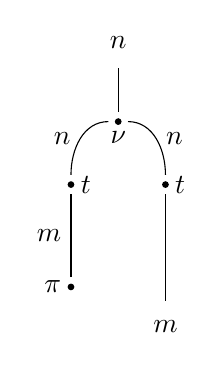
\begin{tikzpicture}
\def\dx{0.6}
\def\dy{0.8}

\def\xa{0};
\def\xb{\dx};
\def\xc{2 * \dx};
\def\xd{3.5 * \dx}

\def \ya{0};
\def \yb{\dy};
\def \yc{2 * \dy};
\def \yd{3 * \dy};
\def \ye{4 * \dy};

\node(a) at (\xa, \yb - 0.5) {};
\node(b) at (\xc, \ya) {};
\node(c) at (\xa, \yc) {};
\node(d) at (\xc, \yc) {};
\node(e) at (\xb, \yd) {};
\node(f) at (\xb, \ye) {};

\filldraw[black] (a) circle (1 pt);
\filldraw[black] (c) circle (1 pt);
\filldraw[black] (d) circle (1 pt);
\filldraw[black] (e) circle (1 pt);

\node [left] at (a) {$\pi$};
\node [right] at (c) {$t$};
\node [right] at (d) {$t$};
\node [below] at (e) {$\nu$};

\draw (a) --  node[left] {$m$} (c);
\draw (b) -- (d);
\draw (c) to [out=90, in=180]  node[left] {$n$} (e);
\draw (d) to [out=90, in=0]   node[right] {$n$} (e);
\draw (e) -- (f);
\node[below] at (b) {$m$};
\node[above] at (f) {$n$};

\end{tikzpicture}
\caption{Path around Fig. \ref{fig-uni2} as a string diagram}
\label{fig-pathup}
\end{figure}

First, let's use the preservation of unit by $t$, Fig. \ref{fig-unitt}, to shrink the left leg,

\begin{figure}[H]
\centering
\begin{tikzpicture}
\def\dx{0.8}
\def\dy{0.8}

\def\xa{0};

\def \ya{0};
\def \yb{\dy};
\def \yc{2 * \dy};
\def \yd{3 * \dy};

\node(a) at (\xa, \ya) {};
\node(b) at (\xa, \yb) {};
\node(c) at (\xa, \yc) {};
\node(d) at (\xa, \yd) {};

\filldraw[black] (b) circle (1 pt);
\filldraw[black] (c) circle (1 pt);

\node [below] at (b) {$\pi$};
\node [right] at (c) {$t$};

\draw (b) --  node[left] {$m$} (c);
\draw (c) -- (d);
\node[above] at (d) {$n$};

\node at (1, \yc) {$=$};

\def\xb{2};

\node(aa) at (\xb, \ya) {};
\node(bb) at (\xb, \yb) {};
\node(cc) at (\xb, \yc) {};
\node(dd) at (\xb, \yd) {};

\filldraw[black] (bb) circle (1 pt);
\node [below] at (bb) {$\eta$};

\node[above] at (dd) {$n$};

\draw (bb) -- (dd);

\end{tikzpicture}
\caption{Preservation of unit by $t$}
\label{fig-unitt}
\end{figure}

and follow it with the left unit law for the monoid $(n, \eta, \nu)$ (Fig. \ref{fig-lunitn}). The result is that Fig. \ref{fig-pathup} shrinks to the single morphism $t$, thus making Fig. \ref{fig-uni2} commute. 

\begin{figure}[H]
\centering
\begin{tikzpicture}
\def\dx{0.6}
\def\xa{0};
\def\xb{\dx};
\def\xc{\dx * 2};

\def \ya{0.8};
\def \yb{1.7};
\def \yc{2.6};

\node(a) at (\xa, \ya) {};
\node(b) at (\xb, \yb) {};
\node(c) at (\xc, 0) {};
\node(d) at (\xb, \yc) {};
\filldraw[black] (a) circle (1 pt);
\node [below] at (a) {$\eta$};
\filldraw[black] (b) circle (1 pt);
\node [below] at (b) {$\nu$};
\draw (a) to [out=90, in=180]  node[left] {$n$}(b);
\draw (c) to [out=90, in=0]  node[right] {$n$} (b);
\draw (b) -- node[right] {$n$} (d);

\def\xd{3.2}
\def\xe{2.3}
\node(e) at (\xd, 0) {};
\node(f) at (\xd, \yc) {};
\node at (\xe, 1.5) {$=$};
\draw (e) -- node[right] {$n$} (f);
\end{tikzpicture}
\caption{Left unit law for the monoid $n$}
\label{fig-lunitn}
\end{figure}
This completes the proof that $t$ is a monoid morphism.


The final step is to make sure that $t$ is the \textit{unique} monoid morphism from $m$ to $n$. Suppose that there is another monoid morphism $t'$ (replacing $t$ in Fig. \ref{fig-freemonalg}). If we can show that $t'$ is also an $h$-algebra morphism induced by the same $\eta$, it will have to, by universality, be equal to $t$. In other words, we have to show that the diagram in Fig. \ref{fig-freemonalg} also works for $t'$. Our assumptions are that both $t$ and $t'$ are monoid morphisms, that is, they preserve unit and multiplication; and they both satisfy the universal condition in Fig \ref{fig-freemon}. In particular, $t'$ satisfies the condition in Fig. \ref{fig-struni2}.


\begin{figure}[H]
\centering
\begin{tikzpicture}
\def\dx{0.6}
\def\xa{0};
\def\xb{\dx};
\def\xc{\dx * 2};

\def\dy{0.8}
\def \ya{0};
\def \yb{\dy};
\def \yc{2 * \dy};
\def \yd{3 * \dy};
\def \ye{4 * \dy};

\node(h) at (\xb, \ya) {};
\node(pi) at (\xc, \yb) {};
\node(sigma) at (\xc, \yc) {};
\node(t) at (\xc, \yd) {};
\node(n) at (\xc, \ye) {};
\filldraw[black] (pi) circle (1 pt);
\filldraw[black] (sigma) circle (1 pt);
\filldraw[black] (t) circle (1 pt);
\node [below] at (h) {$h$};
\node [below] at (pi) {$\pi$};
\node [below left] at (sigma) {$\sigma$};
\node [left] at (t) {$t'$};
\node [above] at (n) {$n$};

\draw (h) to [out=90, in=180] (sigma);
\draw (pi) --  node[right] {$m$} (sigma);
\draw (sigma) -- node[right] {$m$} (t);
\draw (t) -- (n);

\def\xd{2.2}
\def\xe{3.2}
\node at (\xd, 1.5) {$=$};
\node(h2) at (\xe, 0) {};
\node(f) at (\xe, \yc) {};
\node(n2) at (\xe, \ye) {};
\filldraw[black] (f) circle (1 pt);
\node [left] at (f) {$s$};
\draw (h2) -- (f);
\draw (f) -- (n2);
\node [below] at (h2) {$h$};
\node [above] at (n2) {$n$};
\end{tikzpicture}
\caption{Free monoid universal condition for $t'$ as a string diagram}
\label{fig-struni2}
\end{figure}


Notice that, in the first part of the proof, we started with an $h$-algebra morphism $t$ and had to show that it's a monoid morphism. Now we are going in the opposite direction: we know that $t'$ is a monoid morphism, and have to show that it's an $h$-algebra morphism, and that the universal condition in Fig. \ref{fig-freemonalg}
\[t' \circ \pi = \eta\]
holds. The latter simply restates our assumption that $t'$ preserves the unit. 

To show that $t'$ is an algebra morphism, we have to show that the diagram in Fig \ref{fig-halgmor1} commutes.

\begin{figure}[H]
\centering
\begin{tikzcd}
  h \otimes m
  \arrow[rr, "\sigma"]
  \arrow[d, "h \otimes t'"']
  & & m
  \arrow[d, "t'"] \\
  h \otimes n
  \arrow[rr, bend right=40, "\lambda"]
  \arrow[r, "f \otimes n"']
  & n \otimes n
  \arrow[r, "\nu"']
  & n
\end{tikzcd}
\caption{$t'$ as an $h$-algebra morphism}
\label{fig-halgmor1}
\end{figure}
This diagram may be redrawn as a pair of string diagrams, Fig \ref{fig-algmon2}.

\begin{figure}[H]
\centering
\begin{tikzpicture}
\def\dx{0.6}
\def\dy{0.8}

\def\xa{0};
\def\xb{\dx};
\def\xc{2 * \dx};

\def \ya{0};
\def \yb{\dy};
\def \yc{2 * \dy};
\def \yd{3 * \dy};

\node(a) at (\xa, \ya) {};
\node(b) at (\xc, \ya) {};
\node(c) at (\xa, \yb) {};
\node(d) at (\xc, \yb) {};
\node(e) at (\xb, \yc) {};
\node(f) at (\xb, \yd) {};

\filldraw[black] (c) circle (1 pt);
\filldraw[black] (d) circle (1 pt);
\filldraw[black] (e) circle (1 pt);

\node [left] at (c) {$s$};
\node [right] at (d) {$t'$};
\node [below] at (e) {$\nu$};

\draw (a) -- (c);
\draw (b) -- (d);
\draw (c) to [out=90, in=180]  node[left] {$n$} (e);
\draw (d) to [out=90, in=0]   node[right] {$n$} (e);
\draw (e) -- (f);
\node[below] at (a) {$h$};
\node[below] at (b) {$m$};
\node[above] at (f) {$n$};

\def\yy{\yb + 0.5 * \dy}
\node at (2.2, \yy) {$=$};

\def\xx{3}

\def\xxa{\xx};
\def\xxb{\xx + \xb};
\def\xxc{\xx + \xc};

\node(aa) at (\xxa, \ya) {};
\node(bb) at (\xxc, \ya) {};
\node(cc) at (\xxa, \yb) {};
\node(dd) at (\xxc, \yb) {};
\node(ee) at (\xxc, \yb) {};
\node(ff) at (\xxc, \yd) {};
\node(gg) at (\xxc, \yc) {};

\filldraw[black] (ee) circle (1 pt);
\filldraw[black] (gg) circle (1 pt);

\node [right] at (gg) {$t'$};
\node [below left] at (ee) {$\sigma$};

\draw (aa) to [out=90, in=180] (ee);
\draw (bb) -- (ee);
\draw (ee) -- node[right] {$m$} (gg);
\draw (gg) -- (ff);
\node[below] at (aa) {$h$};
\node[below] at (bb) {$m$};
\node[above] at (ff) {$n$};

\end{tikzpicture}
\caption{$t'$ as an algebra morphism}
\label{fig-algmon2}
\end{figure}
The proof of this identity relies on redrawing string diagrams using the identities in Figs. \ref{fig-lunit}, \ref{fig-mualgmor}, \ref{fig-presmul}, and \ref{fig-struni2}. Before we continue, you might want to try it yourself. It's an exercise well worth the effort. 

We start by expanding the $s$ node using the diagram in Fig. \ref{fig-struni2} to get Fig. \ref{fig-struni3}.

\begin{figure}[H]
\centering
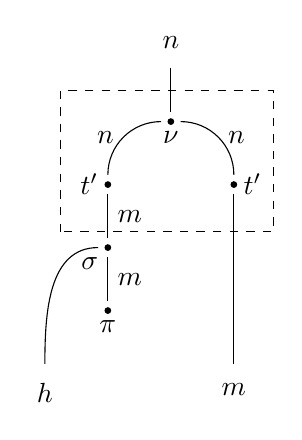
\begin{tikzpicture}
\def\dx{0.8}
\def\xa{0};
\def\xb{\dx};
\def\xc{\dx * 2};
\def\xd{\dx * 4};
\def\xe{\dx * 3};

\def\dy{0.8}
\def \ya{0};
\def \yb{\dy};
\def \yc{2 * \dy};
\def \yd{3 * \dy};
\def \ye{4 * \dy};
\def \yf{5 * \dy};

\node(a) at (\xb, \ya) {};
\node(b) at (\xc, \yb) {};
\node(c) at (\xc, \yc) {};
\node(d) at (\xc, \yd) {};
\node(dr) at (\xd, \yd) {};
\node(e) at (\xe, \ye) {};
\node(f) at (\xd, \ya) {};
\node(g) at (\xe, \yf) {};

\filldraw[black] (b) circle (1 pt);
\filldraw[black] (c) circle (1 pt);
\filldraw[black] (d) circle (1 pt);
\filldraw[black] (dr) circle (1 pt);
\filldraw[black] (e) circle (1 pt);
\node [below] at (a) {$h$};
\node [below] at (b) {$\pi$};
\node [below left] at (c) {$\sigma$};
\node [below] at (f) {$m$};
\node [left] at (d) {$t'$};
\node [right] at (dr) {$t'$};
\node [above] at (g) {$n$};
\node [below] at (e) {$\nu$};
\draw (a) to [out=90, in=180] (c);
\draw (b) --  node[right] {$m$} (c);
\draw (c) -- node[right] {$m$} (d);
\draw (d) to [out=90, in=180] node[left] {$n$}  (e);
\draw (dr) to [out=90, in=0] node[right] {$n$} (e);
\draw (f) -- (dr);
\draw (e) -- (g);

\draw[dashed] (\xb + 0.2, \yc + 0.2) rectangle (\xd + 0.5, \ye + 0.4);

\end{tikzpicture}
\caption{After expanding the left leg of the diagram in Fig. \ref{fig-algmon2}, we can apply preservation of multiplication by $t'$.}
\label{fig-struni3}
\end{figure}

We can now use the preservation of multiplication by $t'$ to obtain Fig \ref{fig-struni4}.

\begin{figure}[H]
\centering
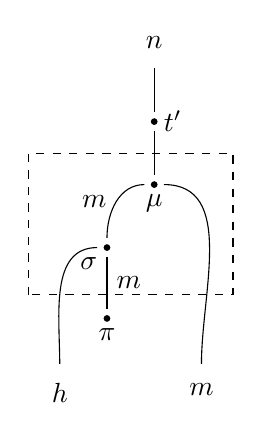
\begin{tikzpicture}
\def\dx{0.6}
\def\xa{0};
\def\xb{\dx};
\def\xc{\dx * 2};
\def\xd{\dx * 4};
\def\xe{\dx * 3};

\def\dy{0.8}
\def \ya{0};
\def \yb{\dy};
\def \yc{2 * \dy};
\def \yd{3 * \dy};
\def \ye{4 * \dy};
\def \yf{5 * \dy};

\node(h) at (\xb, \ya) {};
\node(pi) at (\xc, \yb - 0.1) {};
\node(sigma) at (\xc, \yc) {};
\node(mu) at (\xe, \yd) {};
\node(m) at (\xd, \ya) {};
\node(t) at (\xe, \ye) {};
\node(n) at (\xe, \yf) {};

\filldraw[black] (pi) circle (1 pt);
\filldraw[black] (sigma) circle (1 pt);
\filldraw[black] (mu) circle (1 pt);
\filldraw[black] (t) circle (1 pt);
\node [below] at (h) {$h$};
\node [below] at (pi) {$\pi$};
\node [below left] at (sigma) {$\sigma$};
\node [below] at (m) {$m$};
\node [above] at (n) {$n$};
\node [right] at (t) {$t'$};
\node [below] at (mu) {$\mu$};
\draw (h) to [out=90, in=180] (sigma);
\draw (pi) --  node[right] {$m$} (sigma);
\draw (sigma) to [out=90, in=180] node[left] {$m$}  (mu);
\draw (m) to [out=90, in=0] (mu);
\draw (mu) -- (t);
\draw (t) -- (n);

\draw[dashed] (\xa + 0.2, \yb + 0.2) rectangle (\xd + 0.4, \yd + 0.4);

\end{tikzpicture}
\caption{Applying the fact that $\mu$ is an $h$-algebra morphism}
\label{fig-struni4}
\end{figure}

Next, we can use the fact that $\mu$ is an $h$-algebra morphism, Fig. \ref{fig-mualgmor}, to slide the $\sigma$ node up, and obtain Fig. \ref{fig-struni5}.

\begin{figure}[H]
\centering
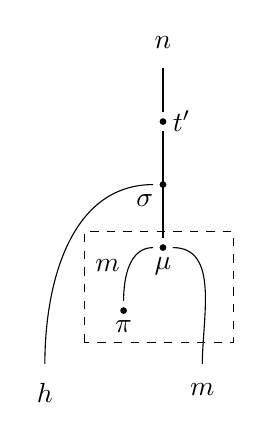
\begin{tikzpicture}
\def\dx{0.5}
\def\xa{0};
\def\xb{\dx};
\def\xc{\dx * 2};
\def\xd{\dx * 4};
\def\xe{\dx * 3};

\def\dy{0.8}
\def \ya{0};
\def \yb{\dy};
\def \yc{2 * \dy};
\def \yd{3 * \dy};
\def \ye{4 * \dy};
\def \yf{5 * \dy};

\node(h) at (\xa, \ya) {};
\node(pi) at (\xc, \yb) {};
\node(sigma) at (\xe, \yd) {};
\node(mu) at (\xe, \yc) {};
\node(m) at (\xd, \ya) {};
\node(t) at (\xe, \ye) {};
\node(n) at (\xe, \yf) {};

\filldraw[black] (pi) circle (1 pt);
\filldraw[black] (sigma) circle (1 pt);
\filldraw[black] (mu) circle (1 pt);
\filldraw[black] (t) circle (1 pt);
\node [below] at (h) {$h$};
\node [below] at (pi) {$\pi$};
\node [below left] at (sigma) {$\sigma$};
\node [below] at (m) {$m$};
\node [above] at (n) {$n$};
\node [right] at (t) {$t'$};
\node [below] at (mu) {$\mu$};

\draw (h) to [out=90, in=180] (sigma);
\draw (pi) to [out=90, in=180] node[left] {$m$}  (mu);
\draw (m) to [out=90, in=0] (mu);
\draw (mu) -- (t);
\draw (t) -- (n);

\draw[dashed] (\xb, \ya + 0.4) rectangle (\xd + 0.4, \yc + 0.2);

\end{tikzpicture}
\caption{Applying left unit law}
\label{fig-struni5}
\end{figure}



We can now use the left unit law for the monoid $m$:
\[\mu \circ (\pi \otimes m) = id\] 
as illustrated in Fig. \ref{fig-lunit}, to arrive at the right hand side of Fig. \ref{fig-algmon2}.

This concludes the proof that $t'$ must be equal to $t$. 

\end{proof}

\subsection{Conclusion}

To summarize, we have shown that the free monoid can be constructed from a free algebra of the functor $h \otimes -$. This is a very general result that is valid in any monoidal closed category. Earlier we've seen that this free algebra is also the initial algebra of the list functor $I + h \otimes -$. The immediate consequence of this theorem is that it lets us construct free monoids in functor categories with interesting monoidal structures. In particular, we get a free monad as a free monoid in the category of endofunctors with functor composition as tensor product. We can also get a free applicative, or free lax monoidal functor, if we define the tensor product as Day convolution---the latter can be also constructed in the profunctor category. 


\begin{thebibliography}{99}
\bibitem{Kelly} Kelly, G.M. “A Unified Treatment of Transfinite Constructions for Free Algebras, Free Monoids, Colimits, Associated Sheaves, and so On.” Bulletin of the Australian Mathematical Society, vol. 22, no. 01, 1980, p. 1., doi:10.1017/s0004972700006353.
\end{thebibliography}

 


\end{document}
